% Options for packages loaded elsewhere
\PassOptionsToPackage{unicode}{hyperref}
\PassOptionsToPackage{hyphens}{url}
\documentclass[
]{article}
\usepackage{xcolor}
\usepackage[margin=1in]{geometry}
\usepackage{amsmath,amssymb}
\setcounter{secnumdepth}{-\maxdimen} % remove section numbering
\usepackage{iftex}
\ifPDFTeX
  \usepackage[T1]{fontenc}
  \usepackage[utf8]{inputenc}
  \usepackage{textcomp} % provide euro and other symbols
\else % if luatex or xetex
  \usepackage{unicode-math} % this also loads fontspec
  \defaultfontfeatures{Scale=MatchLowercase}
  \defaultfontfeatures[\rmfamily]{Ligatures=TeX,Scale=1}
\fi
\usepackage{lmodern}
\ifPDFTeX\else
  % xetex/luatex font selection
\fi
% Use upquote if available, for straight quotes in verbatim environments
\IfFileExists{upquote.sty}{\usepackage{upquote}}{}
\IfFileExists{microtype.sty}{% use microtype if available
  \usepackage[]{microtype}
  \UseMicrotypeSet[protrusion]{basicmath} % disable protrusion for tt fonts
}{}
\makeatletter
\@ifundefined{KOMAClassName}{% if non-KOMA class
  \IfFileExists{parskip.sty}{%
    \usepackage{parskip}
  }{% else
    \setlength{\parindent}{0pt}
    \setlength{\parskip}{6pt plus 2pt minus 1pt}}
}{% if KOMA class
  \KOMAoptions{parskip=half}}
\makeatother
\usepackage{color}
\usepackage{fancyvrb}
\newcommand{\VerbBar}{|}
\newcommand{\VERB}{\Verb[commandchars=\\\{\}]}
\DefineVerbatimEnvironment{Highlighting}{Verbatim}{commandchars=\\\{\}}
% Add ',fontsize=\small' for more characters per line
\usepackage{framed}
\definecolor{shadecolor}{RGB}{248,248,248}
\newenvironment{Shaded}{\begin{snugshade}}{\end{snugshade}}
\newcommand{\AlertTok}[1]{\textcolor[rgb]{0.94,0.16,0.16}{#1}}
\newcommand{\AnnotationTok}[1]{\textcolor[rgb]{0.56,0.35,0.01}{\textbf{\textit{#1}}}}
\newcommand{\AttributeTok}[1]{\textcolor[rgb]{0.13,0.29,0.53}{#1}}
\newcommand{\BaseNTok}[1]{\textcolor[rgb]{0.00,0.00,0.81}{#1}}
\newcommand{\BuiltInTok}[1]{#1}
\newcommand{\CharTok}[1]{\textcolor[rgb]{0.31,0.60,0.02}{#1}}
\newcommand{\CommentTok}[1]{\textcolor[rgb]{0.56,0.35,0.01}{\textit{#1}}}
\newcommand{\CommentVarTok}[1]{\textcolor[rgb]{0.56,0.35,0.01}{\textbf{\textit{#1}}}}
\newcommand{\ConstantTok}[1]{\textcolor[rgb]{0.56,0.35,0.01}{#1}}
\newcommand{\ControlFlowTok}[1]{\textcolor[rgb]{0.13,0.29,0.53}{\textbf{#1}}}
\newcommand{\DataTypeTok}[1]{\textcolor[rgb]{0.13,0.29,0.53}{#1}}
\newcommand{\DecValTok}[1]{\textcolor[rgb]{0.00,0.00,0.81}{#1}}
\newcommand{\DocumentationTok}[1]{\textcolor[rgb]{0.56,0.35,0.01}{\textbf{\textit{#1}}}}
\newcommand{\ErrorTok}[1]{\textcolor[rgb]{0.64,0.00,0.00}{\textbf{#1}}}
\newcommand{\ExtensionTok}[1]{#1}
\newcommand{\FloatTok}[1]{\textcolor[rgb]{0.00,0.00,0.81}{#1}}
\newcommand{\FunctionTok}[1]{\textcolor[rgb]{0.13,0.29,0.53}{\textbf{#1}}}
\newcommand{\ImportTok}[1]{#1}
\newcommand{\InformationTok}[1]{\textcolor[rgb]{0.56,0.35,0.01}{\textbf{\textit{#1}}}}
\newcommand{\KeywordTok}[1]{\textcolor[rgb]{0.13,0.29,0.53}{\textbf{#1}}}
\newcommand{\NormalTok}[1]{#1}
\newcommand{\OperatorTok}[1]{\textcolor[rgb]{0.81,0.36,0.00}{\textbf{#1}}}
\newcommand{\OtherTok}[1]{\textcolor[rgb]{0.56,0.35,0.01}{#1}}
\newcommand{\PreprocessorTok}[1]{\textcolor[rgb]{0.56,0.35,0.01}{\textit{#1}}}
\newcommand{\RegionMarkerTok}[1]{#1}
\newcommand{\SpecialCharTok}[1]{\textcolor[rgb]{0.81,0.36,0.00}{\textbf{#1}}}
\newcommand{\SpecialStringTok}[1]{\textcolor[rgb]{0.31,0.60,0.02}{#1}}
\newcommand{\StringTok}[1]{\textcolor[rgb]{0.31,0.60,0.02}{#1}}
\newcommand{\VariableTok}[1]{\textcolor[rgb]{0.00,0.00,0.00}{#1}}
\newcommand{\VerbatimStringTok}[1]{\textcolor[rgb]{0.31,0.60,0.02}{#1}}
\newcommand{\WarningTok}[1]{\textcolor[rgb]{0.56,0.35,0.01}{\textbf{\textit{#1}}}}
\usepackage{graphicx}
\makeatletter
\newsavebox\pandoc@box
\newcommand*\pandocbounded[1]{% scales image to fit in text height/width
  \sbox\pandoc@box{#1}%
  \Gscale@div\@tempa{\textheight}{\dimexpr\ht\pandoc@box+\dp\pandoc@box\relax}%
  \Gscale@div\@tempb{\linewidth}{\wd\pandoc@box}%
  \ifdim\@tempb\p@<\@tempa\p@\let\@tempa\@tempb\fi% select the smaller of both
  \ifdim\@tempa\p@<\p@\scalebox{\@tempa}{\usebox\pandoc@box}%
  \else\usebox{\pandoc@box}%
  \fi%
}
% Set default figure placement to htbp
\def\fps@figure{htbp}
\makeatother
\setlength{\emergencystretch}{3em} % prevent overfull lines
\providecommand{\tightlist}{%
  \setlength{\itemsep}{0pt}\setlength{\parskip}{0pt}}
\usepackage{booktabs}
\usepackage{longtable}
\usepackage{array}
\usepackage{multirow}
\usepackage{wrapfig}
\usepackage{float}
\usepackage{colortbl}
\usepackage{pdflscape}
\usepackage{tabu}
\usepackage{threeparttable}
\usepackage{threeparttablex}
\usepackage[normalem]{ulem}
\usepackage{makecell}
\usepackage{xcolor}
\usepackage{bookmark}
\IfFileExists{xurl.sty}{\usepackage{xurl}}{} % add URL line breaks if available
\urlstyle{same}
\hypersetup{
  pdftitle={Models of vegetation composition based on climate predictors},
  pdfauthor={Alice Stears},
  hidelinks,
  pdfcreator={LaTeX via pandoc}}

\title{Models of vegetation composition based on climate predictors}
\usepackage{etoolbox}
\makeatletter
\providecommand{\subtitle}[1]{% add subtitle to \maketitle
  \apptocmd{\@title}{\par {\large #1 \par}}{}{}
}
\makeatother
\subtitle{Based on code from Martin Holdrege's Sagebrush-Fire paper}
\author{Alice Stears}
\date{2025-03-21}

\begin{document}
\maketitle

{
\setcounter{tocdepth}{2}
\tableofcontents
}
The data consists of vegetation \% cover by functional group from across
CONUS (from AIM, FIA, LANDFIRE, and RAP), as well as climate variables
from DayMet, which have been aggregated into mean interannual conditions
accross multiple temporal windows.

\section{Dependencies}\label{dependencies}

User defined parameters

\begin{Shaded}
\begin{Highlighting}[]
\FunctionTok{print}\NormalTok{(params)}
\end{Highlighting}
\end{Shaded}

\begin{verbatim}
## $run
## [1] FALSE
## 
## $test_run
## [1] FALSE
## 
## $save_figs
## [1] FALSE
## 
## $ecoregion
## [1] "shrubGrass"
## 
## $response
## [1] "TotalHerbaceousCover"
## 
## $hmod
## [1] FALSE
## 
## $s
## [1] "TotalHerbaceousCover"
## 
## $sample_group
## [1] 1
## 
## $byRegion
## [1] TRUE
\end{verbatim}

\begin{Shaded}
\begin{Highlighting}[]
\CommentTok{\# set to true if want to run for a limited number of rows (i.e. for code testing)}
\NormalTok{test\_run }\OtherTok{\textless{}{-}}\NormalTok{ params}\SpecialCharTok{$}\NormalTok{test\_run}
\NormalTok{save\_figs }\OtherTok{\textless{}{-}}\NormalTok{ params}\SpecialCharTok{$}\NormalTok{save\_figs}
\NormalTok{hmod }\OtherTok{\textless{}{-}}\NormalTok{ params}\SpecialCharTok{$}\NormalTok{hmod }\CommentTok{\# whether to include human modification in the model}
\CommentTok{\# by changing the sample\_group the model can be fit to a completely different set of rows}
\NormalTok{sample\_group }\OtherTok{\textless{}{-}}\NormalTok{ params}\SpecialCharTok{$}\NormalTok{sample\_group }
\NormalTok{response }\OtherTok{\textless{}{-}}\NormalTok{ params}\SpecialCharTok{$}\NormalTok{response}
\CommentTok{\# \_ann defines this model as being built on annual data}
\NormalTok{s }\OtherTok{\textless{}{-}}\NormalTok{ params}\SpecialCharTok{$}\NormalTok{s }\CommentTok{\# string to paste to file names e.g., that defines the interactions in the model}
\CommentTok{\# such as (summer ppt * MAT) and annuals*temperature interactions}
\NormalTok{fit\_sample }\OtherTok{\textless{}{-}} \ConstantTok{TRUE} \CommentTok{\# fit model to a sample of the data}
\NormalTok{n\_train }\OtherTok{\textless{}{-}} \FloatTok{5e4} \CommentTok{\# sample size of the training data}
\NormalTok{n\_test }\OtherTok{\textless{}{-}} \FloatTok{1e6} \CommentTok{\# sample size of the testing data (if this is too big the decile dotplot code throws memory errors)}
\NormalTok{byRegion }\OtherTok{\textless{}{-}}\NormalTok{ params}\SpecialCharTok{$}\NormalTok{byRegion}

\NormalTok{run }\OtherTok{\textless{}{-}}\NormalTok{ params}\SpecialCharTok{$}\NormalTok{run}
\end{Highlighting}
\end{Shaded}

\begin{Shaded}
\begin{Highlighting}[]
\CommentTok{\# set option so resampled dataset created here reproduces earlier runs of this code with dplyr 1.0.10}
\FunctionTok{source}\NormalTok{(}\StringTok{"../../../Functions/glmTransformsIterates.R"}\NormalTok{)}
\FunctionTok{source}\NormalTok{(}\StringTok{"../../../Functions/transformPreds.R"}\NormalTok{)}
\FunctionTok{source}\NormalTok{(}\StringTok{"../../../Functions/StepBeta\_mine.R"}\NormalTok{)}
\CommentTok{\#source("src/fig\_params.R")}
\CommentTok{\#source("src/modeling\_functions.R")}
\FunctionTok{library}\NormalTok{(glinternet)}
\FunctionTok{library}\NormalTok{(terra)}
\FunctionTok{library}\NormalTok{(tidyterra)}
\FunctionTok{library}\NormalTok{(sf)}
\FunctionTok{library}\NormalTok{(caret)}
\FunctionTok{library}\NormalTok{(tidyverse)}
\FunctionTok{library}\NormalTok{(GGally) }\CommentTok{\# for ggpairs()}
\FunctionTok{library}\NormalTok{(pdp) }\CommentTok{\# for partial dependence plots}
\FunctionTok{library}\NormalTok{(gridExtra)}
\FunctionTok{library}\NormalTok{(knitr)}
\FunctionTok{library}\NormalTok{(patchwork) }\CommentTok{\# for figure insets etc. }
\FunctionTok{library}\NormalTok{(ggtext)}
\FunctionTok{library}\NormalTok{(StepBeta)}
\FunctionTok{theme\_set}\NormalTok{(}\FunctionTok{theme\_classic}\NormalTok{())}
\FunctionTok{library}\NormalTok{(here)}
\FunctionTok{library}\NormalTok{(rsample)}
\FunctionTok{library}\NormalTok{(kableExtra)}
\FunctionTok{library}\NormalTok{(glmnet)}
\end{Highlighting}
\end{Shaded}

\section{read in data}\label{read-in-data}

Data compiled in the \texttt{prepDataForModels.R} script

\begin{Shaded}
\begin{Highlighting}[]
\NormalTok{here}\SpecialCharTok{::}\FunctionTok{i\_am}\NormalTok{(}\StringTok{"Analysis/VegComposition/ModelFitting/01\_PredictorVarSelection.Rmd"}\NormalTok{)}
\NormalTok{modDat }\OtherTok{\textless{}{-}} \FunctionTok{readRDS}\NormalTok{( }\FunctionTok{here}\NormalTok{(}\StringTok{"Data\_processed"}\NormalTok{, }\StringTok{"CoverData"}\NormalTok{, }\StringTok{"DataForModels\_spatiallyAveraged\_withSoils\_noSf.rds"}\NormalTok{))}
\DocumentationTok{\#\# there are some values of the annual wet degree days 5th percentile that have {-}Inf?? change to lowest value for now? }
\NormalTok{modDat[}\FunctionTok{is.infinite}\NormalTok{(modDat}\SpecialCharTok{$}\NormalTok{annWetDegDays\_5percentile\_3yrAnom), }\StringTok{"annWetDegDays\_5percentile\_3yrAnom"}\NormalTok{] }\OtherTok{\textless{}{-}} \SpecialCharTok{{-}}\FloatTok{47.8}
\DocumentationTok{\#\# same, but for annual water deficit 95th percentile }
\NormalTok{modDat[}\FunctionTok{is.infinite}\NormalTok{(modDat}\SpecialCharTok{$}\NormalTok{annWaterDeficit\_95percentile\_3yrAnom), }\StringTok{"annWaterDeficit\_95percentile\_3yrAnom"}\NormalTok{] }\OtherTok{\textless{}{-}} \SpecialCharTok{{-}}\DecValTok{600}

\CommentTok{\# \# Convert total cover variables into proportions (for later use in beta regression models) ... proportions are already scaled from zero to 1}
\CommentTok{\# modDat \textless{}{-} modDat \%\textgreater{}\%}
\CommentTok{\#   mutate(TotalTreeCover = TotalTreeCover/100,}
\CommentTok{\#          CAMCover = CAMCover/100,}
\CommentTok{\#          TotalHerbaceousCover = TotalHerbaceousCover/100,}
\CommentTok{\#          BareGroundCover = BareGroundCover/100,}
\CommentTok{\#          ShrubCover = ShrubCover/100}
\CommentTok{\#          )}
\CommentTok{\# For all response variables, make sure there are no 0s add or subtract .0001 from each, since the Gamma model framework can\textquotesingle{}t handle that}
\NormalTok{modDat[modDat}\SpecialCharTok{$}\NormalTok{TotalTreeCover }\SpecialCharTok{==} \DecValTok{0} \SpecialCharTok{\&} \SpecialCharTok{!}\FunctionTok{is.na}\NormalTok{(modDat}\SpecialCharTok{$}\NormalTok{TotalTreeCover), }\StringTok{"TotalTreeCover"}\NormalTok{] }\OtherTok{\textless{}{-}} \FloatTok{0.0001}
\NormalTok{modDat[modDat}\SpecialCharTok{$}\NormalTok{CAMCover }\SpecialCharTok{==} \DecValTok{0} \SpecialCharTok{\&} \SpecialCharTok{!}\FunctionTok{is.na}\NormalTok{(modDat}\SpecialCharTok{$}\NormalTok{CAMCover), }\StringTok{"CAMCover"}\NormalTok{] }\OtherTok{\textless{}{-}} \FloatTok{0.0001}
\NormalTok{modDat[modDat}\SpecialCharTok{$}\NormalTok{TotalHerbaceousCover }\SpecialCharTok{==} \DecValTok{0}  \SpecialCharTok{\&} \SpecialCharTok{!}\FunctionTok{is.na}\NormalTok{(modDat}\SpecialCharTok{$}\NormalTok{TotalHerbaceousCover), }\StringTok{"TotalHerbaceousCover"}\NormalTok{] }\OtherTok{\textless{}{-}} \FloatTok{0.0001}
\NormalTok{modDat[modDat}\SpecialCharTok{$}\NormalTok{BareGroundCover }\SpecialCharTok{==} \DecValTok{0} \SpecialCharTok{\&} \SpecialCharTok{!}\FunctionTok{is.na}\NormalTok{(modDat}\SpecialCharTok{$}\NormalTok{BareGroundCover), }\StringTok{"BareGroundCover"}\NormalTok{] }\OtherTok{\textless{}{-}} \FloatTok{0.0001}
\NormalTok{modDat[modDat}\SpecialCharTok{$}\NormalTok{ShrubCover }\SpecialCharTok{==} \DecValTok{0} \SpecialCharTok{\&} \SpecialCharTok{!}\FunctionTok{is.na}\NormalTok{(modDat}\SpecialCharTok{$}\NormalTok{ShrubCover), }\StringTok{"ShrubCover"}\NormalTok{] }\OtherTok{\textless{}{-}} \FloatTok{0.0001}
\NormalTok{modDat[modDat}\SpecialCharTok{$}\NormalTok{BroadleavedTreeCover\_prop }\SpecialCharTok{==} \DecValTok{0} \SpecialCharTok{\&} \SpecialCharTok{!}\FunctionTok{is.na}\NormalTok{(modDat}\SpecialCharTok{$}\NormalTok{BroadleavedTreeCover\_prop), }\StringTok{"BroadleavedTreeCover\_prop"}\NormalTok{] }\OtherTok{\textless{}{-}} \FloatTok{0.0001}
\NormalTok{modDat[modDat}\SpecialCharTok{$}\NormalTok{NeedleLeavedTreeCover\_prop }\SpecialCharTok{==} \DecValTok{0} \SpecialCharTok{\&} \SpecialCharTok{!}\FunctionTok{is.na}\NormalTok{(modDat}\SpecialCharTok{$}\NormalTok{NeedleLeavedTreeCover\_prop), }\StringTok{"NeedleLeavedTreeCover\_prop"}\NormalTok{] }\OtherTok{\textless{}{-}} \FloatTok{0.0001}
\NormalTok{modDat[modDat}\SpecialCharTok{$}\NormalTok{C4Cover\_prop }\SpecialCharTok{==} \DecValTok{0} \SpecialCharTok{\&} \SpecialCharTok{!}\FunctionTok{is.na}\NormalTok{(modDat}\SpecialCharTok{$}\NormalTok{C4Cover\_prop), }\StringTok{"C4Cover\_prop"}\NormalTok{] }\OtherTok{\textless{}{-}} \FloatTok{0.0001}
\NormalTok{modDat[modDat}\SpecialCharTok{$}\NormalTok{C3Cover\_prop }\SpecialCharTok{==} \DecValTok{0} \SpecialCharTok{\&} \SpecialCharTok{!}\FunctionTok{is.na}\NormalTok{(modDat}\SpecialCharTok{$}\NormalTok{C3Cover\_prop), }\StringTok{"C3Cover\_prop"}\NormalTok{] }\OtherTok{\textless{}{-}} \FloatTok{0.0001}
\NormalTok{modDat[modDat}\SpecialCharTok{$}\NormalTok{ForbCover\_prop }\SpecialCharTok{==} \DecValTok{0} \SpecialCharTok{\&} \SpecialCharTok{!}\FunctionTok{is.na}\NormalTok{(modDat}\SpecialCharTok{$}\NormalTok{ForbCover\_prop), }\StringTok{"ForbCover\_prop"}\NormalTok{] }\OtherTok{\textless{}{-}} \FloatTok{0.0001}
\CommentTok{\# }
\CommentTok{\# modDat[modDat$TotalTreeCover ==1\& !is.na(modDat$TotalTreeCover), "TotalTreeCover"] \textless{}{-} 0.999}
\CommentTok{\# modDat[modDat$CAMCover ==1\& !is.na(modDat$CAMCover), "CAMCover"] \textless{}{-} 0.999}
\CommentTok{\# modDat[modDat$TotalHerbaceousCover ==1 \& !is.na(modDat$TotalHerbaceousCover), "TotalHerbaceousCover"] \textless{}{-} 0.999}
\CommentTok{\# modDat[modDat$BareGroundCover ==1\& !is.na(modDat$BareGroundCover), "BareGroundCover"] \textless{}{-} 0.999}
\CommentTok{\# modDat[modDat$ShrubCover ==1\& !is.na(modDat$ShrubCover), "ShrubCover"] \textless{}{-} 0.999}
\CommentTok{\# modDat[modDat$BroadleavedTreeCover\_prop ==1\& !is.na(modDat$BroadleavedTreeCover\_prop), "BroadleavedTreeCover\_prop"] \textless{}{-} 0.999}
\CommentTok{\# modDat[modDat$NeedleLeavedTreeCover\_prop ==1\& !is.na(modDat$NeedleLeavedTreeCover\_prop), "NeedleLeavedTreeCover\_prop"] \textless{}{-} 0.999}
\CommentTok{\# modDat[modDat$C4Cover\_prop ==1\& !is.na(modDat$C4Cover\_prop), "C4Cover\_prop"] \textless{}{-} 0.999}
\CommentTok{\# modDat[modDat$C3Cover\_prop ==1\& !is.na(modDat$C3Cover\_prop), "C3Cover\_prop"] \textless{}{-} 0.999}
\CommentTok{\# modDat[modDat$ForbCover\_prop ==1\& !is.na(modDat$ForbCover\_prop), "ForbCover\_prop"] \textless{}{-} 0.999}
\end{Highlighting}
\end{Shaded}

\section{Prep data}\label{prep-data}

\begin{Shaded}
\begin{Highlighting}[]
\FunctionTok{set.seed}\NormalTok{(}\DecValTok{1234}\NormalTok{)}
\NormalTok{modDat\_1 }\OtherTok{\textless{}{-}}\NormalTok{ modDat }\SpecialCharTok{\%\textgreater{}\%} 
  \FunctionTok{select}\NormalTok{(}\SpecialCharTok{{-}}\FunctionTok{c}\NormalTok{(prcp\_annTotal}\SpecialCharTok{:}\NormalTok{annVPD\_min)) }\SpecialCharTok{\%\textgreater{}\%} 
  \CommentTok{\# mutate(Lon = st\_coordinates(.)[,1], }
  \CommentTok{\#        Lat = st\_coordinates(.)[,2])  \%\textgreater{}\% }
  \CommentTok{\# st\_drop\_geometry() \%\textgreater{}\% }
  \CommentTok{\# filter(!is.na(newRegion))}
  \FunctionTok{rename}\NormalTok{(}\StringTok{"tmin"} \OtherTok{=}\NormalTok{ tmin\_meanAnnAvg\_CLIM, }
     \StringTok{"tmax"} \OtherTok{=}\NormalTok{ tmax\_meanAnnAvg\_CLIM, }\CommentTok{\#1}
     \StringTok{"tmean"} \OtherTok{=}\NormalTok{ tmean\_meanAnnAvg\_CLIM, }
     \StringTok{"prcp"} \OtherTok{=}\NormalTok{ prcp\_meanAnnTotal\_CLIM, }
     \StringTok{"t\_warm"} \OtherTok{=}\NormalTok{ T\_warmestMonth\_meanAnnAvg\_CLIM,}
     \StringTok{"t\_cold"} \OtherTok{=}\NormalTok{ T\_coldestMonth\_meanAnnAvg\_CLIM, }
     \StringTok{"prcp\_wet"} \OtherTok{=}\NormalTok{ precip\_wettestMonth\_meanAnnAvg\_CLIM,}
     \StringTok{"prcp\_dry"} \OtherTok{=}\NormalTok{ precip\_driestMonth\_meanAnnAvg\_CLIM, }
     \StringTok{"prcp\_seasonality"} \OtherTok{=}\NormalTok{ precip\_Seasonality\_meanAnnAvg\_CLIM, }\CommentTok{\#2}
     \StringTok{"prcpTempCorr"} \OtherTok{=}\NormalTok{ PrecipTempCorr\_meanAnnAvg\_CLIM,  }\CommentTok{\#3}
     \StringTok{"abvFreezingMonth"} \OtherTok{=}\NormalTok{ aboveFreezing\_month\_meanAnnAvg\_CLIM, }
     \StringTok{"isothermality"} \OtherTok{=}\NormalTok{ isothermality\_meanAnnAvg\_CLIM, }\CommentTok{\#4}
     \StringTok{"annWatDef"} \OtherTok{=}\NormalTok{ annWaterDeficit\_meanAnnAvg\_CLIM, }
     \StringTok{"annWetDegDays"} \OtherTok{=}\NormalTok{ annWetDegDays\_meanAnnAvg\_CLIM,}
     \StringTok{"VPD\_mean"} \OtherTok{=}\NormalTok{ annVPD\_mean\_meanAnnAvg\_CLIM, }
     \StringTok{"VPD\_max"} \OtherTok{=}\NormalTok{ annVPD\_max\_meanAnnAvg\_CLIM, }\CommentTok{\#5}
     \StringTok{"VPD\_min"} \OtherTok{=}\NormalTok{ annVPD\_min\_meanAnnAvg\_CLIM, }\CommentTok{\#6}
     \StringTok{"VPD\_max\_95"} \OtherTok{=}\NormalTok{ annVPD\_max\_95percentile\_CLIM, }
     \StringTok{"annWatDef\_95"} \OtherTok{=}\NormalTok{ annWaterDeficit\_95percentile\_CLIM, }
     \StringTok{"annWetDegDays\_5"} \OtherTok{=}\NormalTok{ annWetDegDays\_5percentile\_CLIM, }
     \StringTok{"frostFreeDays\_5"} \OtherTok{=}\NormalTok{ durationFrostFreeDays\_5percentile\_CLIM, }
     \StringTok{"frostFreeDays"} \OtherTok{=}\NormalTok{ durationFrostFreeDays\_meanAnnAvg\_CLIM, }
     \StringTok{"soilDepth"} \OtherTok{=}\NormalTok{ soilDepth, }\CommentTok{\#7}
     \StringTok{"clay"} \OtherTok{=}\NormalTok{ surfaceClay\_perc, }
     \StringTok{"sand"} \OtherTok{=}\NormalTok{ avgSandPerc\_acrossDepth, }\CommentTok{\#8}
     \StringTok{"coarse"} \OtherTok{=}\NormalTok{ avgCoarsePerc\_acrossDepth, }\CommentTok{\#9}
     \StringTok{"carbon"} \OtherTok{=}\NormalTok{ avgOrganicCarbonPerc\_0\_3cm, }\CommentTok{\#10}
     \StringTok{"AWHC"} \OtherTok{=}\NormalTok{ totalAvailableWaterHoldingCapacity,}
     \DocumentationTok{\#\# anomaly variables}
     \AttributeTok{tmean\_anom =}\NormalTok{ tmean\_meanAnnAvg\_3yrAnom, }\CommentTok{\#15}
     \AttributeTok{tmin\_anom =}\NormalTok{ tmin\_meanAnnAvg\_3yrAnom, }\CommentTok{\#16}
     \AttributeTok{tmax\_anom =}\NormalTok{ tmax\_meanAnnAvg\_3yrAnom, }\CommentTok{\#17}
    \AttributeTok{prcp\_anom =}\NormalTok{ prcp\_meanAnnTotal\_3yrAnom, }\CommentTok{\#18}
      \AttributeTok{t\_warm\_anom =}\NormalTok{ T\_warmestMonth\_meanAnnAvg\_3yrAnom,  }\CommentTok{\#19}
     \AttributeTok{t\_cold\_anom =}\NormalTok{ T\_coldestMonth\_meanAnnAvg\_3yrAnom, }\CommentTok{\#20}
      \AttributeTok{prcp\_wet\_anom =}\NormalTok{ precip\_wettestMonth\_meanAnnAvg\_3yrAnom, }\CommentTok{\#21}
      \AttributeTok{precp\_dry\_anom =}\NormalTok{ precip\_driestMonth\_meanAnnAvg\_3yrAnom,  }\CommentTok{\#22}
    \AttributeTok{prcp\_seasonality\_anom =}\NormalTok{ precip\_Seasonality\_meanAnnAvg\_3yrAnom, }\CommentTok{\#23 }
     \AttributeTok{prcpTempCorr\_anom =}\NormalTok{ PrecipTempCorr\_meanAnnAvg\_3yrAnom, }\CommentTok{\#24}
      \AttributeTok{aboveFreezingMonth\_anom =}\NormalTok{ aboveFreezing\_month\_meanAnnAvg\_3yrAnom, }\CommentTok{\#25  }
    \AttributeTok{isothermality\_anom =}\NormalTok{ isothermality\_meanAnnAvg\_3yrAnom, }\CommentTok{\#26}
       \AttributeTok{annWatDef\_anom =}\NormalTok{ annWaterDeficit\_meanAnnAvg\_3yrAnom, }\CommentTok{\#27}
     \AttributeTok{annWetDegDays\_anom =}\NormalTok{ annWetDegDays\_meanAnnAvg\_3yrAnom,  }\CommentTok{\#28}
      \AttributeTok{VPD\_mean\_anom =}\NormalTok{ annVPD\_mean\_meanAnnAvg\_3yrAnom, }\CommentTok{\#29}
      \AttributeTok{VPD\_min\_anom =}\NormalTok{ annVPD\_min\_meanAnnAvg\_3yrAnom,  }\CommentTok{\#30}
      \AttributeTok{VPD\_max\_anom =}\NormalTok{ annVPD\_max\_meanAnnAvg\_3yrAnom,  }\CommentTok{\#31}
     \AttributeTok{VPD\_max\_95\_anom =}\NormalTok{ annVPD\_max\_95percentile\_3yrAnom, }\CommentTok{\#32}
      \AttributeTok{annWatDef\_95\_anom =}\NormalTok{ annWaterDeficit\_95percentile\_3yrAnom, }\CommentTok{\#33 }
      \AttributeTok{annWetDegDays\_5\_anom =}\NormalTok{ annWetDegDays\_5percentile\_3yrAnom ,  }\CommentTok{\#34}
    \AttributeTok{frostFreeDays\_5\_anom =}\NormalTok{ durationFrostFreeDays\_5percentile\_3yrAnom, }\CommentTok{\#35 }
      \AttributeTok{frostFreeDays\_anom =}\NormalTok{ durationFrostFreeDays\_meanAnnAvg\_3yrAnom }\CommentTok{\#36}
\NormalTok{  )}

\CommentTok{\# small dataset for if testing the data}
\ControlFlowTok{if}\NormalTok{(test\_run) \{}
\NormalTok{  modDat\_1 }\OtherTok{\textless{}{-}} \FunctionTok{slice\_sample}\NormalTok{(modDat\_1, }\AttributeTok{n =} \FloatTok{1e5}\NormalTok{)}
\NormalTok{\}}
\end{Highlighting}
\end{Shaded}

Identify the ecoregion and response variable type to use in this model
run

\begin{Shaded}
\begin{Highlighting}[]
\NormalTok{ecoregion }\OtherTok{\textless{}{-}}\NormalTok{ params}\SpecialCharTok{$}\NormalTok{ecoregion}
\NormalTok{response }\OtherTok{\textless{}{-}}\NormalTok{ params}\SpecialCharTok{$}\NormalTok{response}
\FunctionTok{print}\NormalTok{(}\FunctionTok{paste0}\NormalTok{(}\StringTok{"In this model run, the ecoregion is "}\NormalTok{, ecoregion,}\StringTok{" and the response variable is "}\NormalTok{,response))}
\end{Highlighting}
\end{Shaded}

\begin{verbatim}
## [1] "In this model run, the ecoregion is shrubGrass and the response variable is TotalHerbaceousCover"
\end{verbatim}

Subset the data to only include data for the ecoregion of interest

\begin{Shaded}
\begin{Highlighting}[]
\ControlFlowTok{if}\NormalTok{ (ecoregion }\SpecialCharTok{==} \StringTok{"shrubGrass"}\NormalTok{) \{}
  \CommentTok{\# select data for the ecoregion of interest}
\NormalTok{  modDat\_1 }\OtherTok{\textless{}{-}}\NormalTok{ modDat\_1 }\SpecialCharTok{\%\textgreater{}\%}
    \FunctionTok{filter}\NormalTok{(newRegion }\SpecialCharTok{==} \StringTok{"dryShrubGrass"}\NormalTok{)}
\NormalTok{\} }\ControlFlowTok{else} \ControlFlowTok{if}\NormalTok{ (ecoregion }\SpecialCharTok{==} \StringTok{"forest"}\NormalTok{) \{}
  \CommentTok{\# select data for the ecoregion of interest}
\NormalTok{  modDat\_1 }\OtherTok{\textless{}{-}}\NormalTok{ modDat\_1 }\SpecialCharTok{\%\textgreater{}\%} 
    \FunctionTok{filter}\NormalTok{(newRegion }\SpecialCharTok{\%in\%} \FunctionTok{c}\NormalTok{(}\StringTok{"eastForest"}\NormalTok{, }\StringTok{"westForest"}\NormalTok{))}
\NormalTok{\}}

\CommentTok{\# remove the rows that have no observations for the response variable of interest}
\NormalTok{modDat\_1 }\OtherTok{\textless{}{-}}\NormalTok{ modDat\_1[}\SpecialCharTok{!}\FunctionTok{is.na}\NormalTok{(modDat\_1[,response]),]}
\end{Highlighting}
\end{Shaded}

\subsection{Visualize the response
variable}\label{visualize-the-response-variable}

\begin{Shaded}
\begin{Highlighting}[]
\FunctionTok{hist}\NormalTok{(modDat\_1[,response], }\AttributeTok{main =} \FunctionTok{paste0}\NormalTok{(}\StringTok{"Histogram of "}\NormalTok{,response),}
     \AttributeTok{xlab =} \FunctionTok{paste0}\NormalTok{(response))}
\end{Highlighting}
\end{Shaded}

\pandocbounded{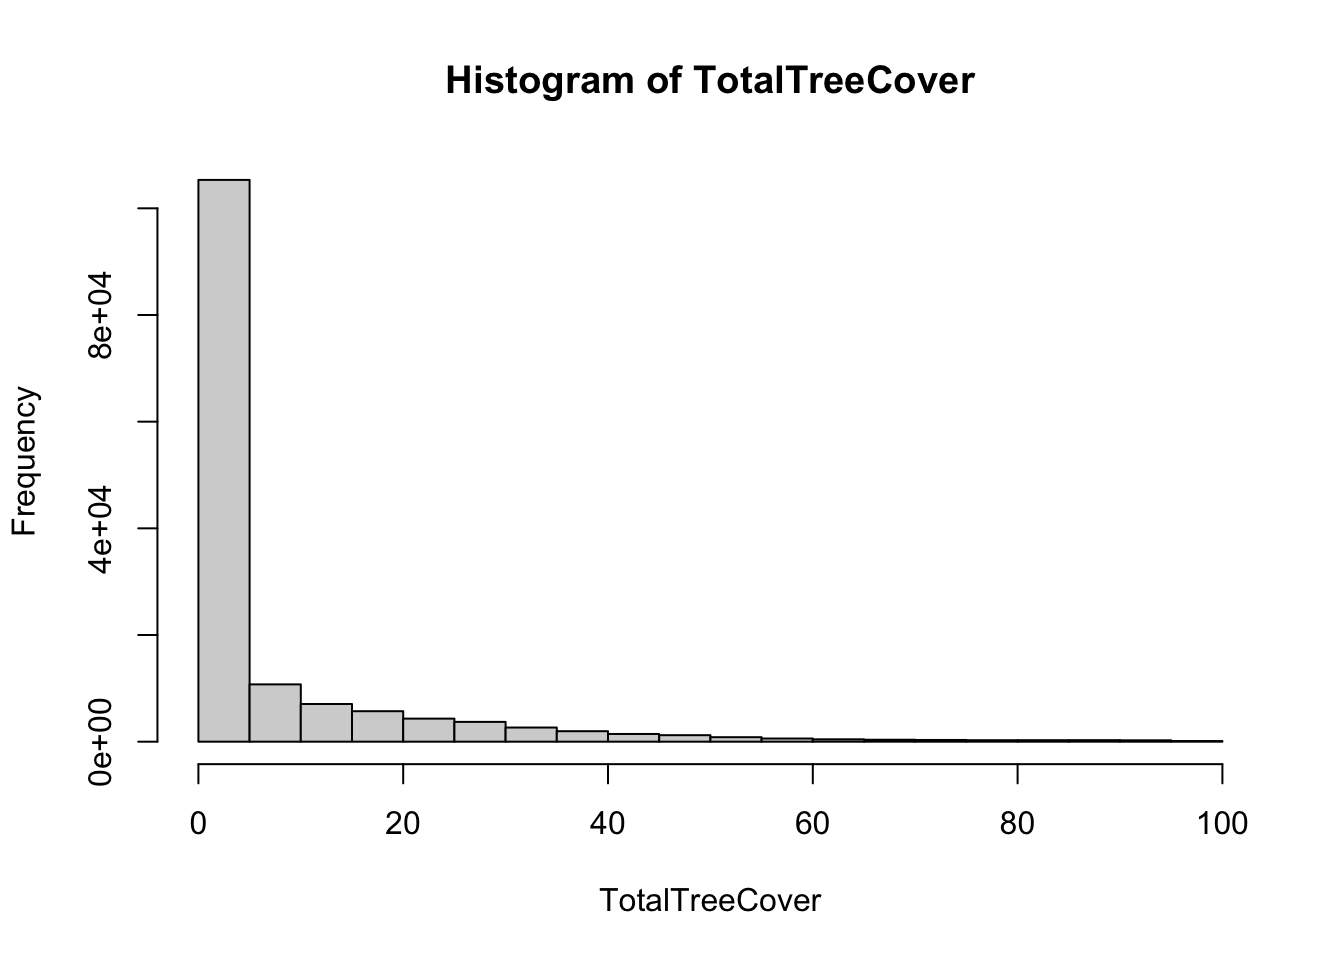
\includegraphics[keepaspectratio]{02_ModelFitting_files/figure-latex/visualize response variable-1.pdf}}

\subsection{Visualize the predictor
variables}\label{visualize-the-predictor-variables}

The following are the candidate predictor variables for this ecoregion:

\begin{Shaded}
\begin{Highlighting}[]
\ControlFlowTok{if}\NormalTok{ (ecoregion }\SpecialCharTok{==} \StringTok{"shrubGrass"}\NormalTok{) \{}
  \CommentTok{\# select potential predictor variables for the ecoregion of interest}
\NormalTok{        prednames }\OtherTok{\textless{}{-}}
          \FunctionTok{c}\NormalTok{(}
\StringTok{"tmean"}\NormalTok{                  , }\StringTok{"prcp"}\NormalTok{               ,}\StringTok{"prcp\_seasonality"}\NormalTok{     ,}\StringTok{"prcpTempCorr"}\NormalTok{        ,   }
\StringTok{"isothermality"}\NormalTok{          , }\StringTok{"VPD\_max"}\NormalTok{            ,}\StringTok{"sand"}\NormalTok{                 ,}\StringTok{"coarse"}\NormalTok{              ,   }
\StringTok{"AWHC"}\NormalTok{                   , }\StringTok{"tmax\_anom"}\NormalTok{          ,}\StringTok{"t\_warm\_anom"}\NormalTok{          ,}\StringTok{"t\_cold\_anom"}\NormalTok{         ,   }
\StringTok{"prcp\_wet\_anom"}\NormalTok{          , }\StringTok{"precp\_dry\_anom"}\NormalTok{     ,}\StringTok{"prcp\_seasonality\_anom"}\NormalTok{,}\StringTok{"prcpTempCorr\_anom"}\NormalTok{   ,   }
\StringTok{"aboveFreezingMonth\_anom"}\NormalTok{, }\StringTok{"isothermality\_anom"}\NormalTok{ ,}\StringTok{"annWatDef\_anom"}\NormalTok{       ,}\StringTok{"annWetDegDays\_anom"}\NormalTok{  ,   }
\StringTok{"VPD\_min\_anom"}\NormalTok{           , }\StringTok{"VPD\_max\_95\_anom"}\NormalTok{    ,   }
\StringTok{"frostFreeDays\_5\_anom"}\NormalTok{   )}
  
\NormalTok{\} }\ControlFlowTok{else} \ControlFlowTok{if}\NormalTok{ (ecoregion }\SpecialCharTok{==} \StringTok{"forest"}\NormalTok{) \{}
  \CommentTok{\# select potential predictor variables for the ecoregion of interest}
\NormalTok{  prednames }\OtherTok{\textless{}{-}} 
    \FunctionTok{c}\NormalTok{(}
\StringTok{"tmean"}\NormalTok{               , }\StringTok{"prcp"}\NormalTok{                , }\StringTok{"prcpTempCorr"}\NormalTok{            ,}\StringTok{"isothermality"}\NormalTok{      , }
\StringTok{"annWatDef"}\NormalTok{           , }\StringTok{"annWetDegDays"}\NormalTok{       , }\StringTok{"sand"}\NormalTok{                    ,}\StringTok{"coarse"}\NormalTok{             , }
\StringTok{"carbon"}\NormalTok{              , }\StringTok{"AWHC"}\NormalTok{                , }\StringTok{"tmax\_anom"}\NormalTok{               ,}\StringTok{"prcp\_anom"}\NormalTok{          , }
\StringTok{"t\_warm\_anom"}\NormalTok{         , }\StringTok{"t\_cold\_anom"}\NormalTok{         , }\StringTok{"prcp\_wet\_anom"}\NormalTok{           ,}\StringTok{"precp\_dry\_anom"}\NormalTok{     , }
\StringTok{"prcp\_seasonality\_anom"}\NormalTok{, }\StringTok{"prcpTempCorr\_anom"}\NormalTok{  ,  }\StringTok{"aboveFreezingMonth\_anom"}\NormalTok{, }\StringTok{"isothermality\_anom"}\NormalTok{,  }
\StringTok{"annWatDef\_anom"}\NormalTok{      , }\StringTok{"annWetDegDays\_anom"}\NormalTok{  , }\StringTok{"VPD\_min\_anom"}\NormalTok{            ,}\StringTok{"VPD\_max\_95\_anom"}\NormalTok{    , }
 \StringTok{"frostFreeDays\_5\_anom"}   
\NormalTok{    )}
\NormalTok{\}}

\CommentTok{\# subset the data to only include these predictors, and remove any remaining NAs }
\NormalTok{modDat\_1 }\OtherTok{\textless{}{-}}\NormalTok{ modDat\_1 }\SpecialCharTok{\%\textgreater{}\%} 
  \FunctionTok{select}\NormalTok{(prednames, response, newRegion, Year.x, Long.x, Lat.x, NA\_L1NAME, NA\_L2NAME) }\SpecialCharTok{\%\textgreater{}\%} 
  \FunctionTok{drop\_na}\NormalTok{()}

\FunctionTok{names}\NormalTok{(prednames) }\OtherTok{\textless{}{-}}\NormalTok{ prednames}
\NormalTok{df\_pred }\OtherTok{\textless{}{-}}\NormalTok{ modDat\_1[, prednames]}
\CommentTok{\# }
\CommentTok{\# \# print the list of predictor variables}
\CommentTok{\# knitr::kable(format = "html", data.frame("Possible\_Predictors" = prednames)}
\CommentTok{\# ) \%\textgreater{}\%}
\CommentTok{\#   kable\_styling(bootstrap\_options = c("striped", "hover", "condensed")) }
\end{Highlighting}
\end{Shaded}

\begin{Shaded}
\begin{Highlighting}[]
\NormalTok{create\_summary }\OtherTok{\textless{}{-}} \ControlFlowTok{function}\NormalTok{(df) \{}
\NormalTok{  df }\SpecialCharTok{\%\textgreater{}\%} 
    \FunctionTok{pivot\_longer}\NormalTok{(}\AttributeTok{cols =} \FunctionTok{everything}\NormalTok{(),}
                 \AttributeTok{names\_to =} \StringTok{\textquotesingle{}variable\textquotesingle{}}\NormalTok{) }\SpecialCharTok{\%\textgreater{}\%} 
    \FunctionTok{group\_by}\NormalTok{(variable) }\SpecialCharTok{\%\textgreater{}\%} 
    \FunctionTok{summarise}\NormalTok{(}\FunctionTok{across}\NormalTok{(value, }\AttributeTok{.fns =} \FunctionTok{list}\NormalTok{(}\AttributeTok{mean =} \SpecialCharTok{\textasciitilde{}}\FunctionTok{mean}\NormalTok{(.x, }\AttributeTok{na.rm =} \ConstantTok{TRUE}\NormalTok{), }\AttributeTok{min =} \SpecialCharTok{\textasciitilde{}}\FunctionTok{min}\NormalTok{(.x, }\AttributeTok{na.rm =} \ConstantTok{TRUE}\NormalTok{), }
                                        \AttributeTok{median =} \SpecialCharTok{\textasciitilde{}}\FunctionTok{median}\NormalTok{(.x, }\AttributeTok{na.rm =} \ConstantTok{TRUE}\NormalTok{), }\AttributeTok{max =} \SpecialCharTok{\textasciitilde{}}\FunctionTok{max}\NormalTok{(.x, }\AttributeTok{na.rm =} \ConstantTok{TRUE}\NormalTok{)))) }\SpecialCharTok{\%\textgreater{}\%} 
    \FunctionTok{mutate}\NormalTok{(}\FunctionTok{across}\NormalTok{(}\FunctionTok{where}\NormalTok{(is.numeric), round, }\DecValTok{4}\NormalTok{))}
\NormalTok{\}}

\NormalTok{modDat\_1[prednames] }\SpecialCharTok{\%\textgreater{}\%} 
  \FunctionTok{create\_summary}\NormalTok{() }\SpecialCharTok{\%\textgreater{}\%} 
\NormalTok{  knitr}\SpecialCharTok{::}\FunctionTok{kable}\NormalTok{(}\AttributeTok{caption =} \StringTok{\textquotesingle{}summaries of possible predictor variables\textquotesingle{}}\NormalTok{) }\SpecialCharTok{\%\textgreater{}\%}
\FunctionTok{kable\_styling}\NormalTok{(}\AttributeTok{bootstrap\_options =} \FunctionTok{c}\NormalTok{(}\StringTok{"striped"}\NormalTok{, }\StringTok{"hover"}\NormalTok{, }\StringTok{"condensed"}\NormalTok{)) }
\end{Highlighting}
\end{Shaded}

\begin{longtable}[t]{lrrrr}
\caption{\label{tab:summary_table}summaries of possible predictor variables}\\
\toprule
variable & value\_mean & value\_min & value\_median & value\_max\\
\midrule
AWHC & 12.2829 & 0.0000 & 12.2550 & 33.6937\\
VPD\_max & 1.1685 & 0.8681 & 1.1719 & 1.4393\\
VPD\_max\_95\_anom & 0.0462 & -0.1818 & 0.0408 & 0.6456\\
VPD\_min\_anom & 0.0088 & -0.0951 & 0.0094 & 0.1285\\
aboveFreezingMonth\_anom & 0.0909 & -1.2576 & 0.0714 & 2.2143\\
\addlinespace
annWatDef\_anom & -0.0081 & -5.7194 & 0.0092 & 1.0000\\
annWetDegDays\_anom & 0.0208 & -0.8181 & 0.0225 & 0.6271\\
coarse & 10.6338 & 0.0000 & 8.5570 & 77.8683\\
frostFreeDays\_5\_anom & -18.1015 & -244.0000 & -16.5000 & 55.8000\\
isothermality & -37.8121 & -58.2327 & -37.2684 & -21.6016\\
\addlinespace
isothermality\_anom & -0.6584 & -8.5059 & -0.5781 & 6.0230\\
prcp & 373.0602 & 91.3360 & 345.4797 & 1658.4937\\
prcpTempCorr & -0.0901 & -0.7786 & -0.0662 & 0.6845\\
prcpTempCorr\_anom & 0.0299 & -0.6495 & 0.0408 & 0.5744\\
prcp\_seasonality & 0.9143 & 0.5289 & 0.8894 & 1.7534\\
\addlinespace
prcp\_seasonality\_anom & -0.0231 & -0.8313 & -0.0157 & 0.4743\\
prcp\_wet\_anom & -0.0242 & -1.9576 & 0.0002 & 0.6697\\
precp\_dry\_anom & -0.0921 & -9.0000 & 0.2668 & 1.0000\\
sand & 48.7510 & 0.0000 & 48.2544 & 94.7159\\
t\_cold\_anom & -0.5171 & -4.4875 & -0.6302 & 5.6504\\
\addlinespace
t\_warm\_anom & -0.5008 & -6.3974 & -0.4914 & 2.5623\\
tmax\_anom & -0.2963 & -3.3596 & -0.3122 & 1.7192\\
tmean & 9.4649 & 0.3909 & 8.5910 & 23.7880\\
\bottomrule
\end{longtable}

\begin{Shaded}
\begin{Highlighting}[]
\CommentTok{\# response\_summary \textless{}{-} modDat\_1 \%\textgreater{}\% }
\CommentTok{\#     dplyr::select(\#where(is.numeric), {-}all\_of(pred\_vars),}
\CommentTok{\#       matches(response)) \%\textgreater{}\% }
\CommentTok{\#     create\_summary()}
\CommentTok{\# }
\CommentTok{\# }
\CommentTok{\# kable(response\_summary, }
\CommentTok{\#       caption = \textquotesingle{}summaries of response variables, calculated using paint\textquotesingle{}) \%\textgreater{}\%}
\CommentTok{\# kable\_styling(bootstrap\_options = c("striped", "hover", "condensed")) }
\end{Highlighting}
\end{Shaded}

\subsection{Plot predictor vars against each
other}\label{plot-predictor-vars-against-each-other}

\begin{Shaded}
\begin{Highlighting}[]
\FunctionTok{set.seed}\NormalTok{(}\DecValTok{12011993}\NormalTok{)}
\CommentTok{\# function for colors}
\NormalTok{my\_fn }\OtherTok{\textless{}{-}} \ControlFlowTok{function}\NormalTok{(data, mapping, }\AttributeTok{method=}\StringTok{"p"}\NormalTok{, }\AttributeTok{use=}\StringTok{"pairwise"}\NormalTok{, ...)\{}
  
  \CommentTok{\# grab data}
\NormalTok{  x }\OtherTok{\textless{}{-}} \FunctionTok{eval\_data\_col}\NormalTok{(data, mapping}\SpecialCharTok{$}\NormalTok{x)}
\NormalTok{  y }\OtherTok{\textless{}{-}} \FunctionTok{eval\_data\_col}\NormalTok{(data, mapping}\SpecialCharTok{$}\NormalTok{y)}
  
  \CommentTok{\# calculate correlation}
\NormalTok{  corr }\OtherTok{\textless{}{-}} \FunctionTok{cor}\NormalTok{(x, y, }\AttributeTok{method=}\NormalTok{method, }\AttributeTok{use=}\NormalTok{use)}
  
  \CommentTok{\# calculate colour based on correlation value}
  \CommentTok{\# Here I have set a correlation of minus one to blue, }
  \CommentTok{\# zero to white, and one to red }
  \CommentTok{\# Change this to suit: possibly extend to add as an argument of \textasciigrave{}my\_fn\textasciigrave{}}
\NormalTok{  colFn }\OtherTok{\textless{}{-}} \FunctionTok{colorRampPalette}\NormalTok{(}\FunctionTok{c}\NormalTok{(}\StringTok{"red"}\NormalTok{, }\StringTok{"white"}\NormalTok{, }\StringTok{"blue"}\NormalTok{), }\AttributeTok{interpolate =}\StringTok{\textquotesingle{}spline\textquotesingle{}}\NormalTok{)}
\NormalTok{  fill }\OtherTok{\textless{}{-}} \FunctionTok{colFn}\NormalTok{(}\DecValTok{100}\NormalTok{)[}\FunctionTok{findInterval}\NormalTok{(corr, }\FunctionTok{seq}\NormalTok{(}\SpecialCharTok{{-}}\DecValTok{1}\NormalTok{, }\DecValTok{1}\NormalTok{, }\AttributeTok{length=}\DecValTok{100}\NormalTok{))]}
  
  \FunctionTok{ggally\_cor}\NormalTok{(}\AttributeTok{data =}\NormalTok{ data, }\AttributeTok{mapping =}\NormalTok{ mapping, }\AttributeTok{size =} \FloatTok{2.5}\NormalTok{, }\AttributeTok{stars =} \ConstantTok{FALSE}\NormalTok{, }
             \AttributeTok{digits =} \DecValTok{2}\NormalTok{, }\AttributeTok{colour =} \FunctionTok{I}\NormalTok{(}\StringTok{"black"}\NormalTok{),...) }\SpecialCharTok{+} 
    \FunctionTok{theme\_void}\NormalTok{() }\SpecialCharTok{+}
    \FunctionTok{theme}\NormalTok{(}\AttributeTok{panel.background =} \FunctionTok{element\_rect}\NormalTok{(}\AttributeTok{fill=}\NormalTok{fill))}
  
\NormalTok{\}}
\NormalTok{(corrPlot }\OtherTok{\textless{}{-}}\NormalTok{ modDat\_1 }\SpecialCharTok{\%\textgreater{}\%} 
  \FunctionTok{select}\NormalTok{(prednames) }\SpecialCharTok{\%\textgreater{}\%} 
  \FunctionTok{slice\_sample}\NormalTok{(}\AttributeTok{n =} \FloatTok{5e4}\NormalTok{) }\SpecialCharTok{\%\textgreater{}\%} 
  \CommentTok{\#select({-}matches("\_")) \%\textgreater{}\% }
\FunctionTok{ggpairs}\NormalTok{( }\AttributeTok{upper =} \FunctionTok{list}\NormalTok{(}\AttributeTok{continuous =}\NormalTok{ my\_fn, }\AttributeTok{size =}\NormalTok{ .}\DecValTok{1}\NormalTok{), }\AttributeTok{lower =} \FunctionTok{list}\NormalTok{(}\AttributeTok{continuous =}\NormalTok{ GGally}\SpecialCharTok{::}\FunctionTok{wrap}\NormalTok{(}\StringTok{"points"}\NormalTok{, }\AttributeTok{alpha =} \FloatTok{0.1}\NormalTok{, }\AttributeTok{size=}\FloatTok{0.1}\NormalTok{)), }\AttributeTok{progress =} \ConstantTok{FALSE}\NormalTok{))}
\end{Highlighting}
\end{Shaded}

\pandocbounded{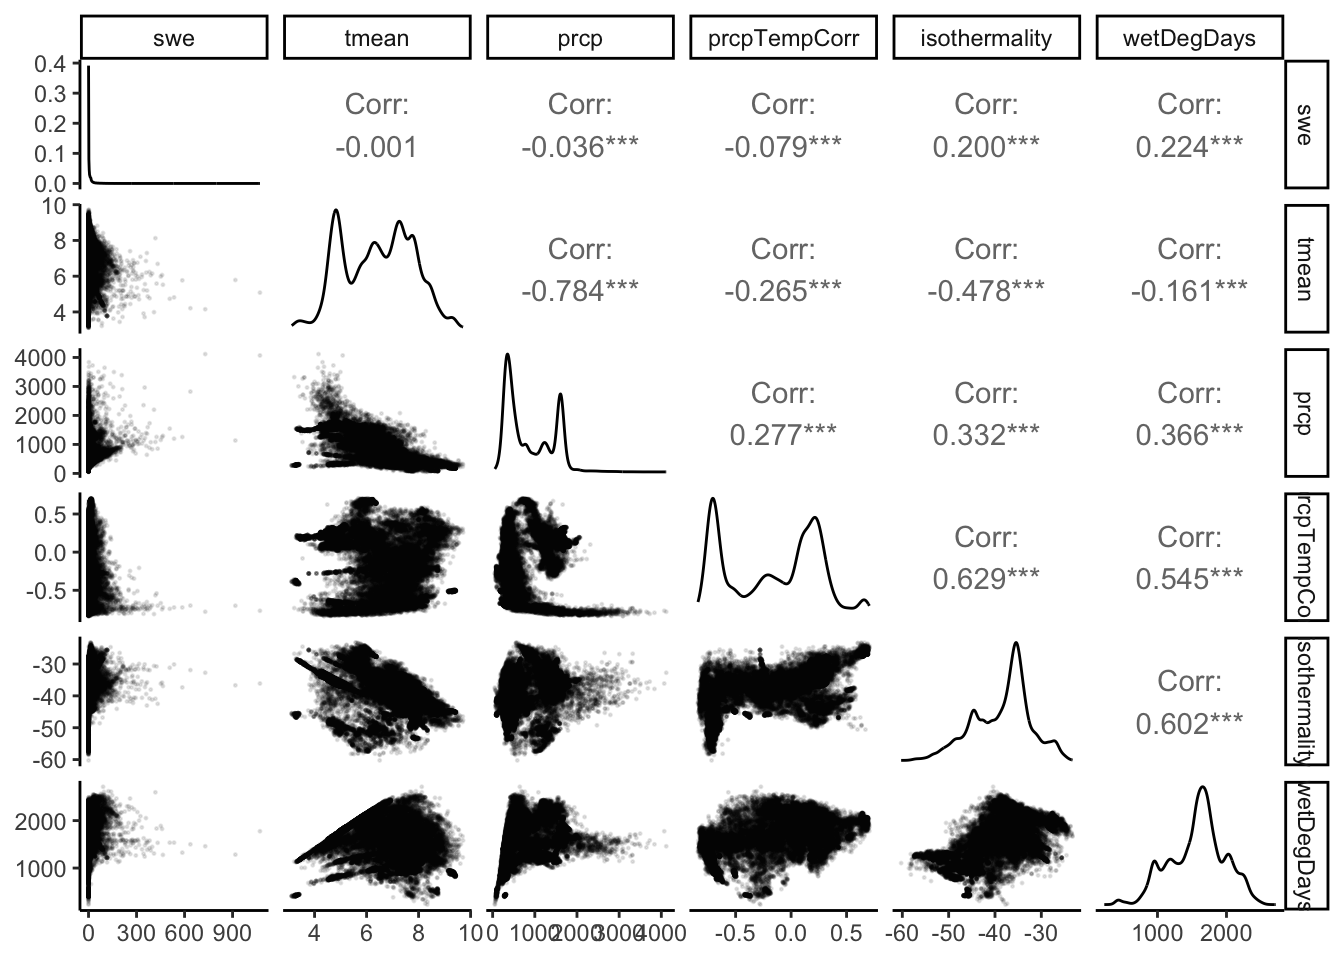
\includegraphics[keepaspectratio]{02_ModelFitting_files/figure-latex/pred_v_pred-1.pdf}}

\subsection{boxplots-- \# predictor variables compared to binned
response
variables}\label{boxplots-predictor-variables-compared-to-binned-response-variables}

\begin{Shaded}
\begin{Highlighting}[]
\FunctionTok{set.seed}\NormalTok{(}\DecValTok{12011993}\NormalTok{)}
\CommentTok{\# vector of name of response variables}
\NormalTok{vars\_response }\OtherTok{\textless{}{-}}\NormalTok{ response}

\CommentTok{\# longformat dataframes for making boxplots}
\NormalTok{df\_sample\_plots }\OtherTok{\textless{}{-}}\NormalTok{  modDat\_1  }\SpecialCharTok{\%\textgreater{}\%} 
  \FunctionTok{slice\_sample}\NormalTok{(}\AttributeTok{n =} \FloatTok{5e4}\NormalTok{) }\SpecialCharTok{\%\textgreater{}\%} 
   \FunctionTok{rename}\NormalTok{(}\AttributeTok{response =} \FunctionTok{all\_of}\NormalTok{(response)) }\SpecialCharTok{\%\textgreater{}\%} 
  \FunctionTok{mutate}\NormalTok{(}\AttributeTok{response =} \FunctionTok{case\_when}\NormalTok{(}
\NormalTok{    response }\SpecialCharTok{\textless{}=}\NormalTok{ .}\DecValTok{25} \SpecialCharTok{\textasciitilde{}} \StringTok{".25"}\NormalTok{, }
\NormalTok{    response }\SpecialCharTok{\textgreater{}}\NormalTok{ .}\DecValTok{25} \SpecialCharTok{\&}\NormalTok{ response }\SpecialCharTok{\textless{}=}\NormalTok{.}\DecValTok{5} \SpecialCharTok{\textasciitilde{}} \StringTok{".5"}\NormalTok{, }
\NormalTok{    response }\SpecialCharTok{\textgreater{}}\NormalTok{ .}\DecValTok{5} \SpecialCharTok{\&}\NormalTok{ response }\SpecialCharTok{\textless{}=}\NormalTok{.}\DecValTok{75} \SpecialCharTok{\textasciitilde{}} \StringTok{".75"}\NormalTok{, }
\NormalTok{    response }\SpecialCharTok{\textgreater{}=}\NormalTok{ .}\DecValTok{75}  \SpecialCharTok{\textasciitilde{}} \StringTok{"1"}\NormalTok{, }
\NormalTok{  )) }\SpecialCharTok{\%\textgreater{}\%} 
  \FunctionTok{select}\NormalTok{(}\FunctionTok{c}\NormalTok{(response, prednames)) }\SpecialCharTok{\%\textgreater{}\%} 
\NormalTok{  tidyr}\SpecialCharTok{::}\FunctionTok{pivot\_longer}\NormalTok{(}\AttributeTok{cols =} \FunctionTok{unname}\NormalTok{(prednames), }
               \AttributeTok{names\_to =} \StringTok{"predictor"}\NormalTok{, }
               \AttributeTok{values\_to =} \StringTok{"value"}
\NormalTok{               )  }
 

  \FunctionTok{ggplot}\NormalTok{(df\_sample\_plots, }\FunctionTok{aes\_string}\NormalTok{(}\AttributeTok{x=} \StringTok{"response"}\NormalTok{, }\AttributeTok{y =} \StringTok{\textquotesingle{}value\textquotesingle{}}\NormalTok{)) }\SpecialCharTok{+}
  \FunctionTok{geom\_boxplot}\NormalTok{() }\SpecialCharTok{+}
  \FunctionTok{facet\_wrap}\NormalTok{(}\SpecialCharTok{\textasciitilde{}}\NormalTok{predictor , }\AttributeTok{scales =} \StringTok{\textquotesingle{}free\_y\textquotesingle{}}\NormalTok{) }\SpecialCharTok{+} 
  \FunctionTok{ylab}\NormalTok{(}\StringTok{"Predictor Variable Values"}\NormalTok{) }\SpecialCharTok{+} 
    \FunctionTok{xlab}\NormalTok{(response)}
\end{Highlighting}
\end{Shaded}

\pandocbounded{\includegraphics[keepaspectratio]{02_ModelFitting_files/figure-latex/climVar_boxplots-1.pdf}}

\section{Model Fitting}\label{model-fitting}

Repeat the following process x \# of times for cross validation {[} 1.
Subset the data into training and test datasets (based on EPA Level II
ecoregion--use leave-one-out CV)

\begin{enumerate}
\def\labelenumi{\arabic{enumi}.}
\setcounter{enumi}{1}
\item
  Then, use cross-validation (based on EPA Level II ecoregion--use
  leave-one-out CV) within the training dataset to identify the
  appropriate regularization parameter
\item
  Then, fit the model with the regularization parameter identified in
  step 2 to the entire training dataset identified in step 1 for this
  iteration
\end{enumerate}

\subsection{First, Fit a null model w/ no
predictors}\label{first-fit-a-null-model-w-no-predictors}

With the full dataset (full response variables) -- use a Gamma family
glm with a ``log'' link function (suited for response variables that are
bounded by 0 and are right skewed)

\begin{Shaded}
\begin{Highlighting}[]
\CommentTok{\# try using bamlss}
\NormalTok{nullMod\_gamma }\OtherTok{\textless{}{-}} \FunctionTok{glm}\NormalTok{(}\AttributeTok{data =}\NormalTok{ modDat\_1, }\AttributeTok{formula =}\NormalTok{ modDat\_1[,response] }\SpecialCharTok{\textasciitilde{}} \DecValTok{1}\NormalTok{, }\AttributeTok{family =}\NormalTok{ stats}\SpecialCharTok{::}\FunctionTok{Gamma}\NormalTok{(}\AttributeTok{link =} \StringTok{"log"}\NormalTok{))}
\CommentTok{\#plot(nullMod\_gamma)}

\FunctionTok{summary}\NormalTok{(nullMod\_gamma)}
\end{Highlighting}
\end{Shaded}

\begin{verbatim}
## 
## Call:
## glm(formula = modDat_1[, response] ~ 1, family = stats::Gamma(link = "log"), 
##     data = modDat_1)
## 
## Coefficients:
##             Estimate Std. Error t value Pr(>|t|)    
## (Intercept) 3.316476   0.004084   812.1   <2e-16 ***
## ---
## Signif. codes:  0 '***' 0.001 '**' 0.01 '*' 0.05 '.' 0.1 ' ' 1
## 
## (Dispersion parameter for Gamma family taken to be 0.8428373)
## 
##     Null deviance: 59369  on 50542  degrees of freedom
## Residual deviance: 59369  on 50542  degrees of freedom
## AIC: 436996
## 
## Number of Fisher Scoring iterations: 6
\end{verbatim}

Visualize the level 2 ecoregions and how they differ across
environmental space

\begin{Shaded}
\begin{Highlighting}[]
\CommentTok{\# make a table of n for each region}
\NormalTok{modDat\_1 }\SpecialCharTok{\%\textgreater{}\%} 
  \FunctionTok{group\_by}\NormalTok{(NA\_L2NAME) }\SpecialCharTok{\%\textgreater{}\%} 
\NormalTok{  dplyr}\SpecialCharTok{::}\FunctionTok{summarize}\NormalTok{(}\StringTok{"Number\_Of\_Observations"} \OtherTok{=} \FunctionTok{length}\NormalTok{(NA\_L2NAME)) }\SpecialCharTok{\%\textgreater{}\%} 
  \FunctionTok{rename}\NormalTok{(}\StringTok{"Level\_2\_Ecoregion"} \OtherTok{=}\NormalTok{ NA\_L2NAME)}\SpecialCharTok{\%\textgreater{}\%} 
  \FunctionTok{kable}\NormalTok{() }\SpecialCharTok{\%\textgreater{}\%}
\FunctionTok{kable\_styling}\NormalTok{(}\AttributeTok{bootstrap\_options =} \FunctionTok{c}\NormalTok{(}\StringTok{"striped"}\NormalTok{, }\StringTok{"hover"}\NormalTok{, }\StringTok{"condensed"}\NormalTok{)) }
\end{Highlighting}
\end{Shaded}

\begin{longtable}[t]{lr}
\toprule
Level\_2\_Ecoregion & Number\_Of\_Observations\\
\midrule
COLD DESERTS & 38371\\
MEDITERRANEAN CALIFORNIA & 373\\
SOUTH CENTRAL SEMIARID PRAIRIES & 1971\\
TAMAULIPAS-TEXAS SEMIARID PLAIN & 34\\
TEMPERATE PRAIRIES & 281\\
\addlinespace
TEXAS-LOUISIANA COASTAL PLAIN & 355\\
WARM DESERTS & 3242\\
WEST-CENTRAL SEMIARID PRAIRIES & 4705\\
WESTERN SIERRA MADRE PIEDMONT & 1211\\
\bottomrule
\end{longtable}

\begin{Shaded}
\begin{Highlighting}[]
\DocumentationTok{\#\# visualize the variation between groups across environmental space}
\DocumentationTok{\#\# make data into spatial format}
\NormalTok{modDat\_1\_sf }\OtherTok{\textless{}{-}}\NormalTok{ modDat\_1 }\SpecialCharTok{\%\textgreater{}\%} 
  \FunctionTok{st\_as\_sf}\NormalTok{(}\AttributeTok{coords =} \FunctionTok{c}\NormalTok{(}\StringTok{"Long.x"}\NormalTok{, }\StringTok{"Lat.x"}\NormalTok{), }\AttributeTok{crs =} \FunctionTok{st\_crs}\NormalTok{(}\StringTok{"PROJCRS[}\SpecialCharTok{\textbackslash{}"}\StringTok{unnamed}\SpecialCharTok{\textbackslash{}"}\StringTok{,}\SpecialCharTok{\textbackslash{}n}\StringTok{    BASEGEOGCRS[}\SpecialCharTok{\textbackslash{}"}\StringTok{unknown}\SpecialCharTok{\textbackslash{}"}\StringTok{,}\SpecialCharTok{\textbackslash{}n}\StringTok{        DATUM[}\SpecialCharTok{\textbackslash{}"}\StringTok{unknown}\SpecialCharTok{\textbackslash{}"}\StringTok{,}\SpecialCharTok{\textbackslash{}n}\StringTok{            ELLIPSOID[}\SpecialCharTok{\textbackslash{}"}\StringTok{Spheroid}\SpecialCharTok{\textbackslash{}"}\StringTok{,6378137,298.257223563,}\SpecialCharTok{\textbackslash{}n}\StringTok{                LENGTHUNIT[}\SpecialCharTok{\textbackslash{}"}\StringTok{metre}\SpecialCharTok{\textbackslash{}"}\StringTok{,1,}\SpecialCharTok{\textbackslash{}n}\StringTok{                    ID[}\SpecialCharTok{\textbackslash{}"}\StringTok{EPSG}\SpecialCharTok{\textbackslash{}"}\StringTok{,9001]]]],}\SpecialCharTok{\textbackslash{}n}\StringTok{        PRIMEM[}\SpecialCharTok{\textbackslash{}"}\StringTok{Greenwich}\SpecialCharTok{\textbackslash{}"}\StringTok{,0,}\SpecialCharTok{\textbackslash{}n}\StringTok{            ANGLEUNIT[}\SpecialCharTok{\textbackslash{}"}\StringTok{degree}\SpecialCharTok{\textbackslash{}"}\StringTok{,0.0174532925199433,}\SpecialCharTok{\textbackslash{}n}\StringTok{                ID[}\SpecialCharTok{\textbackslash{}"}\StringTok{EPSG}\SpecialCharTok{\textbackslash{}"}\StringTok{,9122]]]],}\SpecialCharTok{\textbackslash{}n}\StringTok{    CONVERSION[}\SpecialCharTok{\textbackslash{}"}\StringTok{Lambert Conic Conformal (2SP)}\SpecialCharTok{\textbackslash{}"}\StringTok{,}\SpecialCharTok{\textbackslash{}n}\StringTok{        METHOD[}\SpecialCharTok{\textbackslash{}"}\StringTok{Lambert Conic Conformal (2SP)}\SpecialCharTok{\textbackslash{}"}\StringTok{,}\SpecialCharTok{\textbackslash{}n}\StringTok{            ID[}\SpecialCharTok{\textbackslash{}"}\StringTok{EPSG}\SpecialCharTok{\textbackslash{}"}\StringTok{,9802]],}\SpecialCharTok{\textbackslash{}n}\StringTok{        PARAMETER[}\SpecialCharTok{\textbackslash{}"}\StringTok{Latitude of false origin}\SpecialCharTok{\textbackslash{}"}\StringTok{,42.5,}\SpecialCharTok{\textbackslash{}n}\StringTok{            ANGLEUNIT[}\SpecialCharTok{\textbackslash{}"}\StringTok{degree}\SpecialCharTok{\textbackslash{}"}\StringTok{,0.0174532925199433],}\SpecialCharTok{\textbackslash{}n}\StringTok{            ID[}\SpecialCharTok{\textbackslash{}"}\StringTok{EPSG}\SpecialCharTok{\textbackslash{}"}\StringTok{,8821]],}\SpecialCharTok{\textbackslash{}n}\StringTok{        PARAMETER[}\SpecialCharTok{\textbackslash{}"}\StringTok{Longitude of false origin}\SpecialCharTok{\textbackslash{}"}\StringTok{,{-}100,}\SpecialCharTok{\textbackslash{}n}\StringTok{            ANGLEUNIT[}\SpecialCharTok{\textbackslash{}"}\StringTok{degree}\SpecialCharTok{\textbackslash{}"}\StringTok{,0.0174532925199433],}\SpecialCharTok{\textbackslash{}n}\StringTok{            ID[}\SpecialCharTok{\textbackslash{}"}\StringTok{EPSG}\SpecialCharTok{\textbackslash{}"}\StringTok{,8822]],}\SpecialCharTok{\textbackslash{}n}\StringTok{        PARAMETER[}\SpecialCharTok{\textbackslash{}"}\StringTok{Latitude of 1st standard parallel}\SpecialCharTok{\textbackslash{}"}\StringTok{,25,}\SpecialCharTok{\textbackslash{}n}\StringTok{            ANGLEUNIT[}\SpecialCharTok{\textbackslash{}"}\StringTok{degree}\SpecialCharTok{\textbackslash{}"}\StringTok{,0.0174532925199433],}\SpecialCharTok{\textbackslash{}n}\StringTok{            ID[}\SpecialCharTok{\textbackslash{}"}\StringTok{EPSG}\SpecialCharTok{\textbackslash{}"}\StringTok{,8823]],}\SpecialCharTok{\textbackslash{}n}\StringTok{        PARAMETER[}\SpecialCharTok{\textbackslash{}"}\StringTok{Latitude of 2nd standard parallel}\SpecialCharTok{\textbackslash{}"}\StringTok{,60,}\SpecialCharTok{\textbackslash{}n}\StringTok{            ANGLEUNIT[}\SpecialCharTok{\textbackslash{}"}\StringTok{degree}\SpecialCharTok{\textbackslash{}"}\StringTok{,0.0174532925199433],}\SpecialCharTok{\textbackslash{}n}\StringTok{            ID[}\SpecialCharTok{\textbackslash{}"}\StringTok{EPSG}\SpecialCharTok{\textbackslash{}"}\StringTok{,8824]],}\SpecialCharTok{\textbackslash{}n}\StringTok{        PARAMETER[}\SpecialCharTok{\textbackslash{}"}\StringTok{Easting at false origin}\SpecialCharTok{\textbackslash{}"}\StringTok{,0,}\SpecialCharTok{\textbackslash{}n}\StringTok{            LENGTHUNIT[}\SpecialCharTok{\textbackslash{}"}\StringTok{metre}\SpecialCharTok{\textbackslash{}"}\StringTok{,1],}\SpecialCharTok{\textbackslash{}n}\StringTok{            ID[}\SpecialCharTok{\textbackslash{}"}\StringTok{EPSG}\SpecialCharTok{\textbackslash{}"}\StringTok{,8826]],}\SpecialCharTok{\textbackslash{}n}\StringTok{        PARAMETER[}\SpecialCharTok{\textbackslash{}"}\StringTok{Northing at false origin}\SpecialCharTok{\textbackslash{}"}\StringTok{,0,}\SpecialCharTok{\textbackslash{}n}\StringTok{            LENGTHUNIT[}\SpecialCharTok{\textbackslash{}"}\StringTok{metre}\SpecialCharTok{\textbackslash{}"}\StringTok{,1],}\SpecialCharTok{\textbackslash{}n}\StringTok{            ID[}\SpecialCharTok{\textbackslash{}"}\StringTok{EPSG}\SpecialCharTok{\textbackslash{}"}\StringTok{,8827]]],}\SpecialCharTok{\textbackslash{}n}\StringTok{    CS[Cartesian,2],}\SpecialCharTok{\textbackslash{}n}\StringTok{        AXIS[}\SpecialCharTok{\textbackslash{}"}\StringTok{easting}\SpecialCharTok{\textbackslash{}"}\StringTok{,east,}\SpecialCharTok{\textbackslash{}n}\StringTok{            ORDER[1],}\SpecialCharTok{\textbackslash{}n}\StringTok{            LENGTHUNIT[}\SpecialCharTok{\textbackslash{}"}\StringTok{metre}\SpecialCharTok{\textbackslash{}"}\StringTok{,1,}\SpecialCharTok{\textbackslash{}n}\StringTok{                ID[}\SpecialCharTok{\textbackslash{}"}\StringTok{EPSG}\SpecialCharTok{\textbackslash{}"}\StringTok{,9001]]],}\SpecialCharTok{\textbackslash{}n}\StringTok{        AXIS[}\SpecialCharTok{\textbackslash{}"}\StringTok{northing}\SpecialCharTok{\textbackslash{}"}\StringTok{,north,}\SpecialCharTok{\textbackslash{}n}\StringTok{            ORDER[2],}\SpecialCharTok{\textbackslash{}n}\StringTok{            LENGTHUNIT[}\SpecialCharTok{\textbackslash{}"}\StringTok{metre}\SpecialCharTok{\textbackslash{}"}\StringTok{,1,}\SpecialCharTok{\textbackslash{}n}\StringTok{                ID[}\SpecialCharTok{\textbackslash{}"}\StringTok{EPSG}\SpecialCharTok{\textbackslash{}"}\StringTok{,9001]]]]"}\NormalTok{))}

\NormalTok{us\_states }\OtherTok{\textless{}{-}}\NormalTok{ tigris}\SpecialCharTok{::}\FunctionTok{states}\NormalTok{()}
\end{Highlighting}
\end{Shaded}

\begin{verbatim}
##   |                                                                              |                                                                      |   0%  |                                                                              |                                                                      |   1%  |                                                                              |=                                                                     |   1%  |                                                                              |=                                                                     |   2%  |                                                                              |==                                                                    |   2%  |                                                                              |==                                                                    |   3%  |                                                                              |===                                                                   |   4%  |                                                                              |===                                                                   |   5%  |                                                                              |====                                                                  |   5%  |                                                                              |====                                                                  |   6%  |                                                                              |=====                                                                 |   7%  |                                                                              |=====                                                                 |   8%  |                                                                              |======                                                                |   8%  |                                                                              |======                                                                |   9%  |                                                                              |=======                                                               |   9%  |                                                                              |=======                                                               |  10%  |                                                                              |=======                                                               |  11%  |                                                                              |========                                                              |  11%  |                                                                              |========                                                              |  12%  |                                                                              |=========                                                             |  12%  |                                                                              |=========                                                             |  13%  |                                                                              |==========                                                            |  14%  |                                                                              |==========                                                            |  15%  |                                                                              |===========                                                           |  15%  |                                                                              |===========                                                           |  16%  |                                                                              |============                                                          |  17%  |                                                                              |============                                                          |  18%  |                                                                              |=============                                                         |  18%  |                                                                              |=============                                                         |  19%  |                                                                              |==============                                                        |  19%  |                                                                              |==============                                                        |  20%  |                                                                              |==============                                                        |  21%  |                                                                              |===============                                                       |  21%  |                                                                              |===============                                                       |  22%  |                                                                              |================                                                      |  22%  |                                                                              |================                                                      |  23%  |                                                                              |=================                                                     |  24%  |                                                                              |=================                                                     |  25%  |                                                                              |==================                                                    |  25%  |                                                                              |==================                                                    |  26%  |                                                                              |===================                                                   |  26%  |                                                                              |===================                                                   |  27%  |                                                                              |===================                                                   |  28%  |                                                                              |====================                                                  |  28%  |                                                                              |====================                                                  |  29%  |                                                                              |=====================                                                 |  29%  |                                                                              |=====================                                                 |  30%  |                                                                              |=====================                                                 |  31%  |                                                                              |======================                                                |  31%  |                                                                              |======================                                                |  32%  |                                                                              |=======================                                               |  32%  |                                                                              |=======================                                               |  33%  |                                                                              |=======================                                               |  34%  |                                                                              |========================                                              |  34%  |                                                                              |========================                                              |  35%  |                                                                              |=========================                                             |  35%  |                                                                              |=========================                                             |  36%  |                                                                              |==========================                                            |  36%  |                                                                              |==========================                                            |  37%  |                                                                              |==========================                                            |  38%  |                                                                              |===========================                                           |  38%  |                                                                              |===========================                                           |  39%  |                                                                              |============================                                          |  40%  |                                                                              |============================                                          |  41%  |                                                                              |=============================                                         |  41%  |                                                                              |=============================                                         |  42%  |                                                                              |==============================                                        |  42%  |                                                                              |==============================                                        |  43%  |                                                                              |==============================                                        |  44%  |                                                                              |===============================                                       |  44%  |                                                                              |===============================                                       |  45%  |                                                                              |================================                                      |  45%  |                                                                              |================================                                      |  46%  |                                                                              |=================================                                     |  46%  |                                                                              |=================================                                     |  47%  |                                                                              |=================================                                     |  48%  |                                                                              |==================================                                    |  48%  |                                                                              |==================================                                    |  49%  |                                                                              |===================================                                   |  49%  |                                                                              |===================================                                   |  50%  |                                                                              |===================================                                   |  51%  |                                                                              |====================================                                  |  51%  |                                                                              |====================================                                  |  52%  |                                                                              |=====================================                                 |  52%  |                                                                              |=====================================                                 |  53%  |                                                                              |=====================================                                 |  54%  |                                                                              |======================================                                |  54%  |                                                                              |======================================                                |  55%  |                                                                              |=======================================                               |  55%  |                                                                              |=======================================                               |  56%  |                                                                              |========================================                              |  57%  |                                                                              |========================================                              |  58%  |                                                                              |=========================================                             |  58%  |                                                                              |=========================================                             |  59%  |                                                                              |==========================================                            |  59%  |                                                                              |==========================================                            |  60%  |                                                                              |==========================================                            |  61%  |                                                                              |===========================================                           |  61%  |                                                                              |===========================================                           |  62%  |                                                                              |============================================                          |  62%  |                                                                              |============================================                          |  63%  |                                                                              |============================================                          |  64%  |                                                                              |=============================================                         |  64%  |                                                                              |=============================================                         |  65%  |                                                                              |==============================================                        |  65%  |                                                                              |==============================================                        |  66%  |                                                                              |===============================================                       |  67%  |                                                                              |===============================================                       |  68%  |                                                                              |================================================                      |  68%  |                                                                              |================================================                      |  69%  |                                                                              |=================================================                     |  69%  |                                                                              |=================================================                     |  70%  |                                                                              |=================================================                     |  71%  |                                                                              |==================================================                    |  71%  |                                                                              |==================================================                    |  72%  |                                                                              |===================================================                   |  72%  |                                                                              |===================================================                   |  73%  |                                                                              |====================================================                  |  74%  |                                                                              |====================================================                  |  75%  |                                                                              |=====================================================                 |  75%  |                                                                              |=====================================================                 |  76%  |                                                                              |======================================================                |  77%  |                                                                              |======================================================                |  78%  |                                                                              |=======================================================               |  78%  |                                                                              |=======================================================               |  79%  |                                                                              |========================================================              |  79%  |                                                                              |========================================================              |  80%  |                                                                              |========================================================              |  81%  |                                                                              |=========================================================             |  81%  |                                                                              |=========================================================             |  82%  |                                                                              |==========================================================            |  82%  |                                                                              |==========================================================            |  83%  |                                                                              |===========================================================           |  84%  |                                                                              |===========================================================           |  85%  |                                                                              |============================================================          |  85%  |                                                                              |============================================================          |  86%  |                                                                              |=============================================================         |  87%  |                                                                              |=============================================================         |  88%  |                                                                              |==============================================================        |  88%  |                                                                              |==============================================================        |  89%  |                                                                              |===============================================================       |  90%  |                                                                              |===============================================================       |  91%  |                                                                              |================================================================      |  91%  |                                                                              |================================================================      |  92%  |                                                                              |=================================================================     |  92%  |                                                                              |=================================================================     |  93%  |                                                                              |==================================================================    |  94%  |                                                                              |==================================================================    |  95%  |                                                                              |===================================================================   |  95%  |                                                                              |===================================================================   |  96%  |                                                                              |====================================================================  |  96%  |                                                                              |====================================================================  |  97%  |                                                                              |====================================================================  |  98%  |                                                                              |===================================================================== |  98%  |                                                                              |===================================================================== |  99%  |                                                                              |======================================================================|  99%  |                                                                              |======================================================================| 100%
\end{verbatim}

\begin{Shaded}
\begin{Highlighting}[]
\NormalTok{cropped\_states }\OtherTok{\textless{}{-}}\NormalTok{ us\_states }\SpecialCharTok{\%\textgreater{}\%}
\NormalTok{  dplyr}\SpecialCharTok{::}\FunctionTok{filter}\NormalTok{(NAME}\SpecialCharTok{!=}\StringTok{"Hawaii"}\NormalTok{) }\SpecialCharTok{\%\textgreater{}\%}
\NormalTok{  dplyr}\SpecialCharTok{::}\FunctionTok{filter}\NormalTok{(NAME}\SpecialCharTok{!=}\StringTok{"Alaska"}\NormalTok{) }\SpecialCharTok{\%\textgreater{}\%}
\NormalTok{  dplyr}\SpecialCharTok{::}\FunctionTok{filter}\NormalTok{(NAME}\SpecialCharTok{!=}\StringTok{"Puerto Rico"}\NormalTok{) }\SpecialCharTok{\%\textgreater{}\%}
\NormalTok{  dplyr}\SpecialCharTok{::}\FunctionTok{filter}\NormalTok{(NAME}\SpecialCharTok{!=}\StringTok{"American Samoa"}\NormalTok{) }\SpecialCharTok{\%\textgreater{}\%}
\NormalTok{  dplyr}\SpecialCharTok{::}\FunctionTok{filter}\NormalTok{(NAME}\SpecialCharTok{!=}\StringTok{"Guam"}\NormalTok{) }\SpecialCharTok{\%\textgreater{}\%}
\NormalTok{  dplyr}\SpecialCharTok{::}\FunctionTok{filter}\NormalTok{(NAME}\SpecialCharTok{!=}\StringTok{"Commonwealth of the Northern Mariana Islands"}\NormalTok{) }\SpecialCharTok{\%\textgreater{}\%}
\NormalTok{  dplyr}\SpecialCharTok{::}\FunctionTok{filter}\NormalTok{(NAME}\SpecialCharTok{!=}\StringTok{"United States Virgin Islands"}\NormalTok{) }\SpecialCharTok{\%\textgreater{}\%}

\NormalTok{  sf}\SpecialCharTok{::}\FunctionTok{st\_sf}\NormalTok{() }\SpecialCharTok{\%\textgreater{}\%}
\NormalTok{  sf}\SpecialCharTok{::}\FunctionTok{st\_transform}\NormalTok{(sf}\SpecialCharTok{::}\FunctionTok{st\_crs}\NormalTok{(modDat\_1\_sf)) }\CommentTok{\#\%\textgreater{}\%}
  \CommentTok{\#sf::st\_crop(sf::st\_bbox(modDat\_1\_sf)+c({-}1,{-}1,1,1))}

\NormalTok{map1 }\OtherTok{\textless{}{-}} \FunctionTok{ggplot}\NormalTok{() }\SpecialCharTok{+}
  \FunctionTok{geom\_sf}\NormalTok{(}\AttributeTok{data=}\NormalTok{cropped\_states,}\AttributeTok{fill=}\StringTok{\textquotesingle{}white\textquotesingle{}}\NormalTok{) }\SpecialCharTok{+}
  \FunctionTok{geom\_sf}\NormalTok{(}\AttributeTok{data=}\NormalTok{modDat\_1\_sf,}\FunctionTok{aes}\NormalTok{(}\AttributeTok{fill=}\FunctionTok{as.factor}\NormalTok{(NA\_L2NAME)),}\AttributeTok{linewidth=}\FloatTok{0.5}\NormalTok{,}\AttributeTok{alpha=}\FloatTok{0.5}\NormalTok{) }\SpecialCharTok{+}
  \FunctionTok{geom\_point}\NormalTok{(}\AttributeTok{data=}\NormalTok{modDat\_1,}\AttributeTok{alpha=}\FloatTok{0.5}\NormalTok{, }
             \FunctionTok{aes}\NormalTok{(}\AttributeTok{x =}\NormalTok{ Long.x, }\AttributeTok{y =}\NormalTok{ Lat.x, }\AttributeTok{color=}\FunctionTok{as.factor}\NormalTok{(modDat\_1}\SpecialCharTok{$}\NormalTok{NA\_L2NAME))) }\SpecialCharTok{+}
  \CommentTok{\#scale\_fill\_okabeito() +}
  \CommentTok{\#scale\_color\_okabeito() +}
 \CommentTok{\# theme\_default() +}
  \FunctionTok{theme}\NormalTok{(}\AttributeTok{legend.position =} \StringTok{\textquotesingle{}none\textquotesingle{}}\NormalTok{) }\SpecialCharTok{+}
  \FunctionTok{labs}\NormalTok{(}\AttributeTok{title =} \StringTok{"Level 2 Ecoregions as spatial blocks"}\NormalTok{)}

\NormalTok{hull }\OtherTok{\textless{}{-}}\NormalTok{ modDat\_1\_sf }\SpecialCharTok{\%\textgreater{}\%}
  \FunctionTok{ungroup}\NormalTok{() }\SpecialCharTok{\%\textgreater{}\%}
  \FunctionTok{group\_by}\NormalTok{(NA\_L2NAME) }\SpecialCharTok{\%\textgreater{}\%}
  \FunctionTok{slice}\NormalTok{(}\FunctionTok{chull}\NormalTok{(tmean, prcp))}

\NormalTok{plot1}\OtherTok{\textless{}{-}}\FunctionTok{ggplot}\NormalTok{(}\AttributeTok{data=}\NormalTok{modDat\_1\_sf,}\FunctionTok{aes}\NormalTok{(}\AttributeTok{x=}\NormalTok{tmean,}\AttributeTok{y=}\NormalTok{prcp)) }\SpecialCharTok{+}
  \FunctionTok{geom\_polygon}\NormalTok{(}\AttributeTok{data =}\NormalTok{ hull, }\AttributeTok{alpha =} \FloatTok{0.25}\NormalTok{,}\FunctionTok{aes}\NormalTok{(}\AttributeTok{fill=}\NormalTok{NA\_L2NAME) )}\SpecialCharTok{+}
  \FunctionTok{geom\_point}\NormalTok{(}\FunctionTok{aes}\NormalTok{(}\AttributeTok{group=}\NormalTok{NA\_L2NAME,}\AttributeTok{color=}\NormalTok{NA\_L2NAME),}\AttributeTok{alpha=}\FloatTok{0.25}\NormalTok{) }\SpecialCharTok{+}
  \FunctionTok{theme\_minimal}\NormalTok{() }\SpecialCharTok{+} \FunctionTok{xlab}\NormalTok{(}\StringTok{"Annual Average T\_mean {-} long{-}term average"}\NormalTok{) }\SpecialCharTok{+}
  \FunctionTok{ylab}\NormalTok{(}\StringTok{"Annual Average Precip {-} long{-}term average"}\NormalTok{) }\CommentTok{\#+}
  \CommentTok{\#scale\_color\_okabeito() +}
  \CommentTok{\#scale\_fill\_okabeito()}

\NormalTok{plot2}\OtherTok{\textless{}{-}}\FunctionTok{ggplot}\NormalTok{(}\AttributeTok{data=}\NormalTok{modDat\_1\_sf }\SpecialCharTok{\%\textgreater{}\%}
                \FunctionTok{pivot\_longer}\NormalTok{(}\AttributeTok{cols=}\NormalTok{tmean}\SpecialCharTok{:}\NormalTok{prcp),}
              \FunctionTok{aes}\NormalTok{(}\AttributeTok{x=}\NormalTok{value,}\AttributeTok{group=}\NormalTok{name)) }\SpecialCharTok{+}
  \CommentTok{\# geom\_polygon(data = hull, alpha = 0.25,aes(fill=fold) )+}
  \FunctionTok{geom\_density}\NormalTok{(}\FunctionTok{aes}\NormalTok{(}\AttributeTok{group=}\NormalTok{NA\_L2NAME,}\AttributeTok{fill=}\NormalTok{NA\_L2NAME),}\AttributeTok{alpha=}\FloatTok{0.25}\NormalTok{) }\SpecialCharTok{+}
  \FunctionTok{theme\_minimal}\NormalTok{() }\SpecialCharTok{+}
  \FunctionTok{facet\_wrap}\NormalTok{(}\SpecialCharTok{\textasciitilde{}}\NormalTok{name,}\AttributeTok{scales=}\StringTok{\textquotesingle{}free\textquotesingle{}}\NormalTok{)}\CommentTok{\# +}
  \CommentTok{\#scale\_color\_okabeito() +}
  \CommentTok{\#scale\_fill\_okabeito()}
 
\FunctionTok{library}\NormalTok{(patchwork)}
\NormalTok{(combo }\OtherTok{\textless{}{-}}\NormalTok{ (map1}\SpecialCharTok{+}\NormalTok{plot1)}\SpecialCharTok{/}\NormalTok{plot2) }
\end{Highlighting}
\end{Shaded}

\pandocbounded{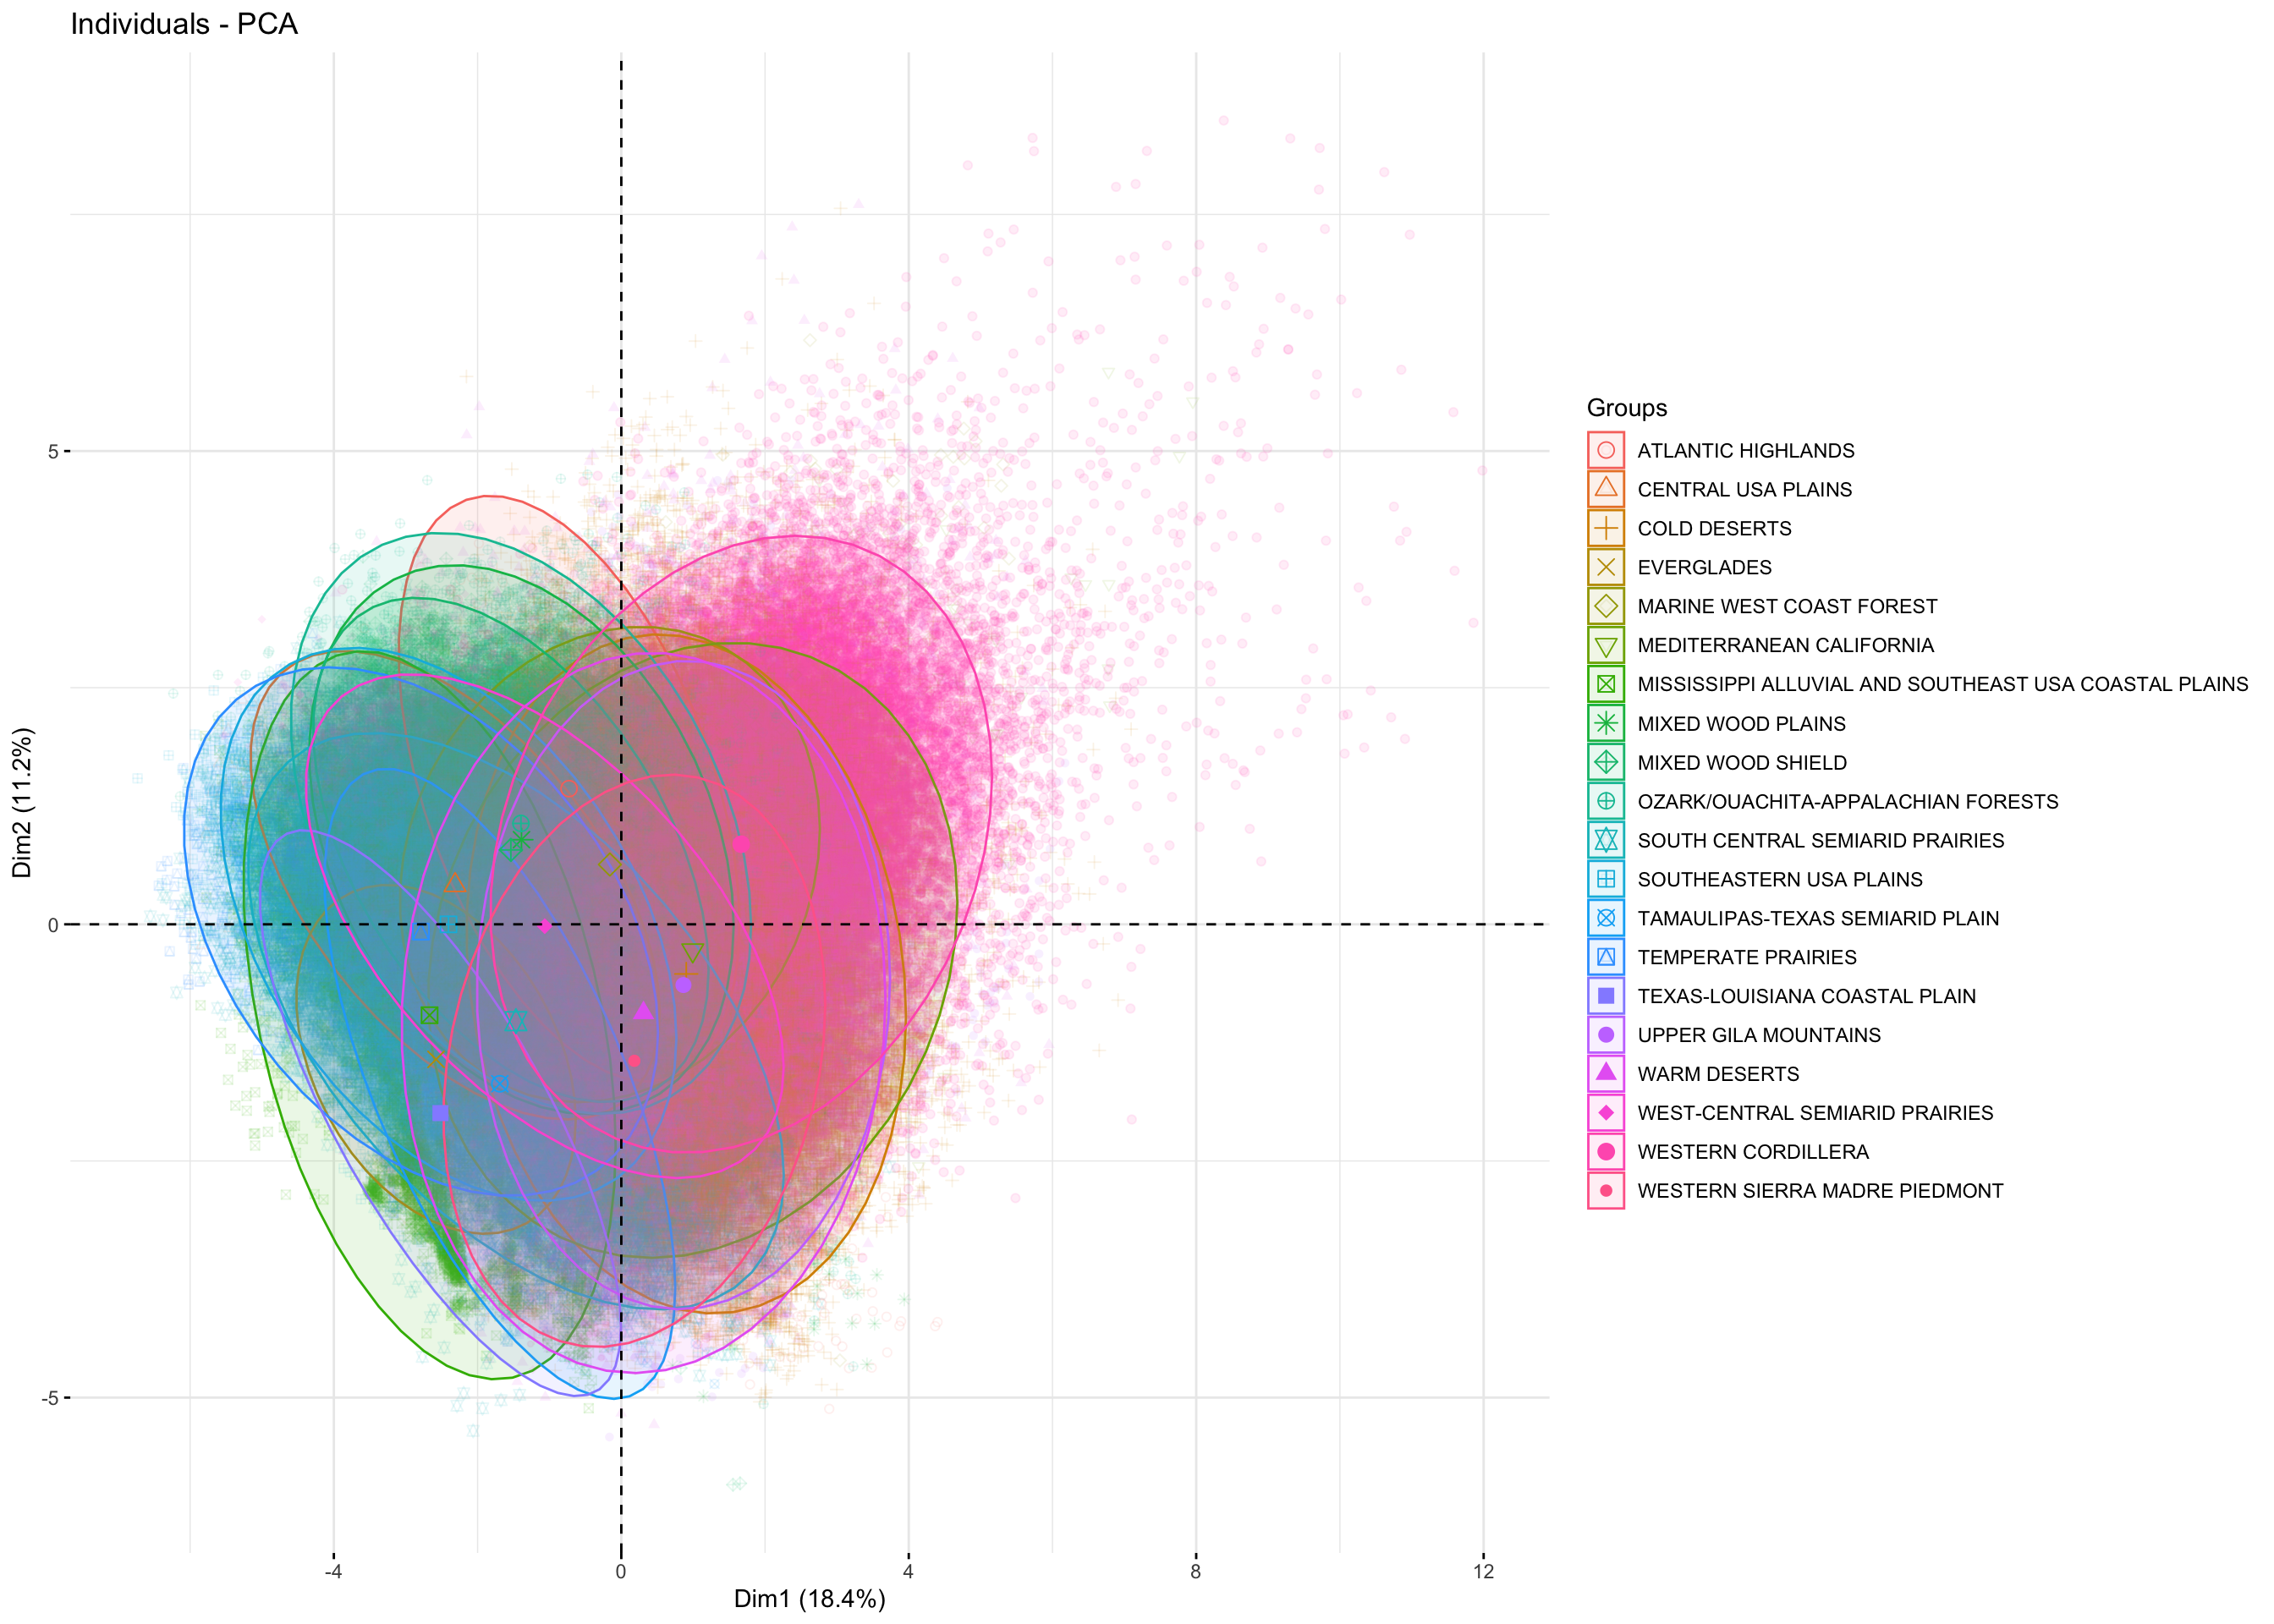
\includegraphics[keepaspectratio]{02_ModelFitting_files/figure-latex/Visualize ecoregion distribution-1.pdf}}

Fit a global model with all of the data -- within the training set, use
level 2 ecoregion for cross-validation to tune lambda in the LASSO model

\begin{verbatim}
## 
## Call:  cv.glmnet(x = X, y = y, lambda = lambdas, type.measure = "mse",      foldid = my_folds, family = stats::Gamma(link = "log"), alpha = 1,      standardize = TRUE) 
## 
## Measure: Mean-Squared Error 
## 
##      Lambda Index Measure    SE Nonzero
## min 0.02833    45   620.9 114.4      33
## 1se 0.08805    31   733.0 104.2       9
\end{verbatim}

\pandocbounded{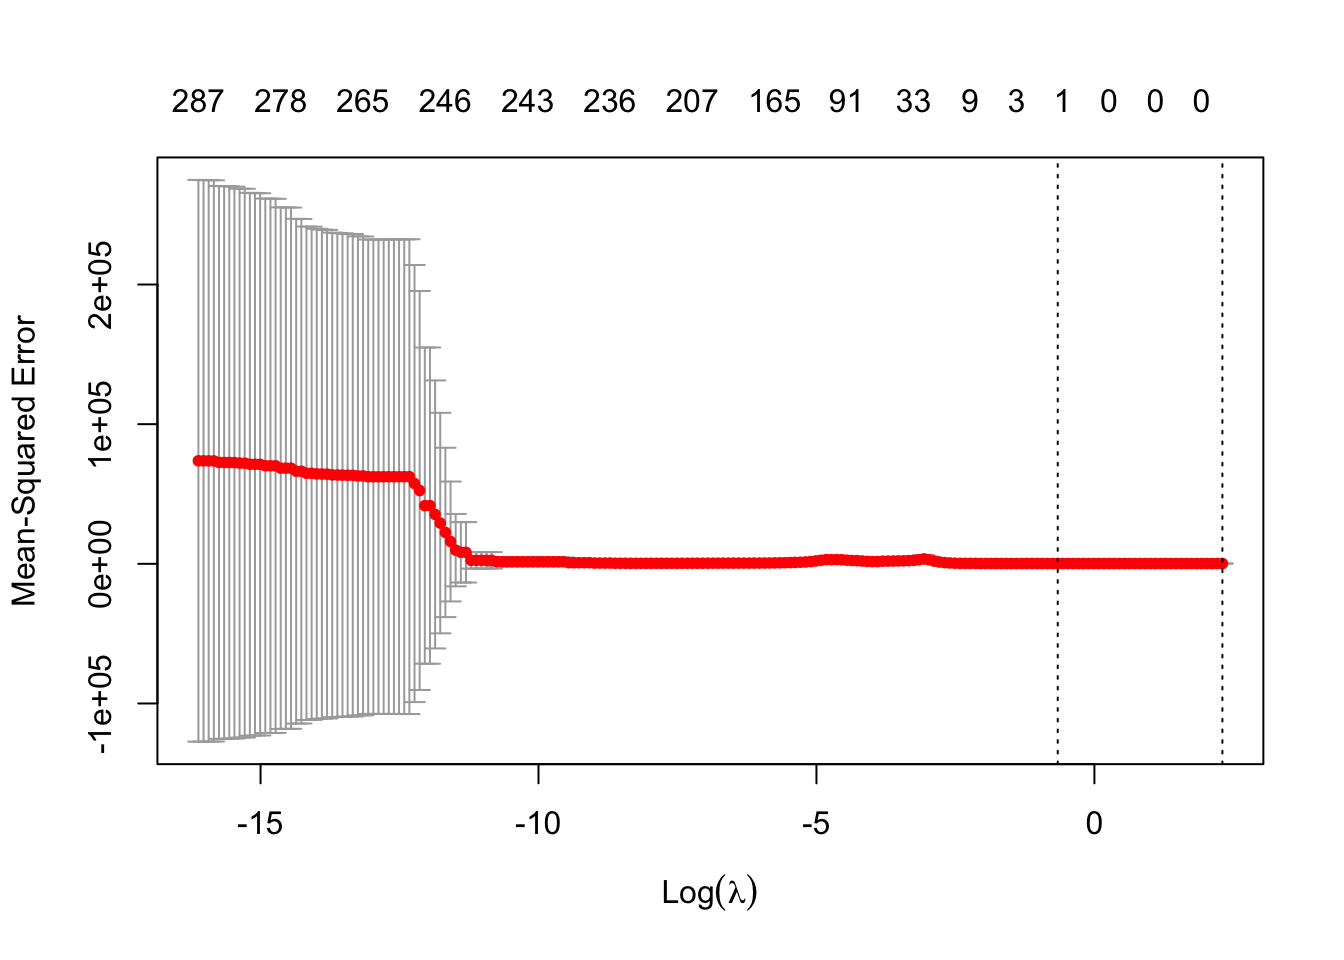
\includegraphics[keepaspectratio]{02_ModelFitting_files/figure-latex/fit global model-1.pdf}}

\begin{verbatim}
## 218 x 1 sparse Matrix of class "dgCMatrix"
##                                                          s1
## (Intercept)                                    2.658883e+00
## (Intercept)                                    .           
## tmean                                          .           
## prcp                                           .           
## prcp_seasonality                               .           
## prcpTempCorr                                   .           
## isothermality                                  6.738948e-02
## VPD_max                                        2.532625e+00
## sand                                          -7.253744e-03
## coarse                                         .           
## AWHC                                           2.066938e-02
## tmax_anom                                      .           
## t_warm_anom                                    .           
## t_cold_anom                                    .           
## prcp_wet_anom                                  .           
## precp_dry_anom                                 .           
## prcp_seasonality_anom                          .           
## prcpTempCorr_anom                              .           
## aboveFreezingMonth_anom                        .           
## isothermality_anom                             .           
## annWatDef_anom                                 .           
## annWetDegDays_anom                             .           
## VPD_min_anom                                   .           
## VPD_max_95_anom                                .           
## frostFreeDays_5_anom                           .           
## aboveFreezingMonth_anom:annWatDef_anom         4.987168e-02
## aboveFreezingMonth_anom:annWetDegDays_anom     .           
## aboveFreezingMonth_anom:frostFreeDays_5_anom   .           
## isothermality:aboveFreezingMonth_anom          .           
## aboveFreezingMonth_anom:isothermality_anom     .           
## prcp:aboveFreezingMonth_anom                   .           
## prcp_seasonality:aboveFreezingMonth_anom       .           
## prcp_seasonality_anom:aboveFreezingMonth_anom  .           
## prcp_wet_anom:aboveFreezingMonth_anom          .           
## prcpTempCorr:aboveFreezingMonth_anom          -1.238290e-01
## prcpTempCorr_anom:aboveFreezingMonth_anom      5.733775e-01
## precp_dry_anom:aboveFreezingMonth_anom         .           
## t_cold_anom:aboveFreezingMonth_anom            7.155751e-02
## t_warm_anom:aboveFreezingMonth_anom            .           
## tmax_anom:aboveFreezingMonth_anom              .           
## tmean:aboveFreezingMonth_anom                  .           
## VPD_max:aboveFreezingMonth_anom                .           
## aboveFreezingMonth_anom:VPD_max_95_anom        .           
## aboveFreezingMonth_anom:VPD_min_anom           .           
## annWatDef_anom:annWetDegDays_anom              .           
## annWatDef_anom:frostFreeDays_5_anom            .           
## isothermality:annWatDef_anom                   .           
## isothermality_anom:annWatDef_anom              .           
## prcp:annWatDef_anom                            .           
## prcp_seasonality:annWatDef_anom                .           
## prcp_seasonality_anom:annWatDef_anom           .           
## prcp_wet_anom:annWatDef_anom                   .           
## prcpTempCorr:annWatDef_anom                    .           
## prcpTempCorr_anom:annWatDef_anom               .           
## precp_dry_anom:annWatDef_anom                  .           
## t_cold_anom:annWatDef_anom                     .           
## t_warm_anom:annWatDef_anom                     .           
## tmax_anom:annWatDef_anom                       .           
## tmean:annWatDef_anom                           .           
## VPD_max:annWatDef_anom                         .           
## annWatDef_anom:VPD_max_95_anom                 .           
## annWatDef_anom:VPD_min_anom                    .           
## annWetDegDays_anom:frostFreeDays_5_anom        .           
## isothermality:annWetDegDays_anom               .           
## isothermality_anom:annWetDegDays_anom          2.035793e-02
## prcp:annWetDegDays_anom                        .           
## prcp_seasonality:annWetDegDays_anom            .           
## prcp_seasonality_anom:annWetDegDays_anom       .           
## prcp_wet_anom:annWetDegDays_anom               .           
## prcpTempCorr:annWetDegDays_anom                .           
## prcpTempCorr_anom:annWetDegDays_anom          -2.134581e-01
## precp_dry_anom:annWetDegDays_anom              .           
## t_cold_anom:annWetDegDays_anom                 .           
## t_warm_anom:annWetDegDays_anom                 4.059460e-02
## tmax_anom:annWetDegDays_anom                   .           
## tmean:annWetDegDays_anom                       .           
## VPD_max:annWetDegDays_anom                     .           
## annWetDegDays_anom:VPD_max_95_anom             .           
## annWetDegDays_anom:VPD_min_anom                .           
## isothermality:frostFreeDays_5_anom             .           
## isothermality_anom:frostFreeDays_5_anom        .           
## prcp:frostFreeDays_5_anom                      .           
## prcp_seasonality:frostFreeDays_5_anom          .           
## prcp_seasonality_anom:frostFreeDays_5_anom     .           
## prcp_wet_anom:frostFreeDays_5_anom             .           
## prcpTempCorr:frostFreeDays_5_anom              .           
## prcpTempCorr_anom:frostFreeDays_5_anom         .           
## precp_dry_anom:frostFreeDays_5_anom            .           
## t_cold_anom:frostFreeDays_5_anom               .           
## t_warm_anom:frostFreeDays_5_anom              -1.325062e-03
## tmax_anom:frostFreeDays_5_anom                 .           
## tmean:frostFreeDays_5_anom                     .           
## VPD_max:frostFreeDays_5_anom                   .           
## VPD_max_95_anom:frostFreeDays_5_anom           .           
## VPD_min_anom:frostFreeDays_5_anom              .           
## isothermality:isothermality_anom               .           
## prcp:isothermality                             .           
## prcp_seasonality:isothermality                 .           
## isothermality:prcp_seasonality_anom            .           
## isothermality:prcp_wet_anom                    .           
## prcpTempCorr:isothermality                    -2.550529e-03
## isothermality:prcpTempCorr_anom                .           
## isothermality:precp_dry_anom                   .           
## isothermality:t_cold_anom                      .           
## isothermality:t_warm_anom                     -2.316551e-04
## isothermality:tmax_anom                        .           
## tmean:isothermality                            .           
## isothermality:VPD_max                          .           
## isothermality:VPD_max_95_anom                  1.330831e-03
## isothermality:VPD_min_anom                     .           
## prcp:isothermality_anom                        .           
## prcp_seasonality:isothermality_anom            .           
## prcp_seasonality_anom:isothermality_anom       .           
## prcp_wet_anom:isothermality_anom               .           
## prcpTempCorr:isothermality_anom                .           
## prcpTempCorr_anom:isothermality_anom           .           
## precp_dry_anom:isothermality_anom              .           
## t_cold_anom:isothermality_anom                -6.082725e-03
## t_warm_anom:isothermality_anom                 .           
## tmax_anom:isothermality_anom                   .           
## tmean:isothermality_anom                       .           
## VPD_max:isothermality_anom                     .           
## isothermality_anom:VPD_max_95_anom             1.571203e-01
## isothermality_anom:VPD_min_anom                .           
## prcp:prcp_seasonality                          8.031168e-04
## prcp:prcp_seasonality_anom                     .           
## prcp:prcp_wet_anom                             .           
## prcp:prcpTempCorr                              .           
## prcp:prcpTempCorr_anom                         .           
## prcp:precp_dry_anom                           -3.612680e-05
## prcp:t_cold_anom                               .           
## prcp:t_warm_anom                               .           
## prcp:tmax_anom                                 .           
## tmean:prcp                                     1.494172e-05
## prcp:VPD_max                                   .           
## prcp:VPD_max_95_anom                           .           
## prcp:VPD_min_anom                              .           
## prcp_seasonality:prcp_seasonality_anom         .           
## prcp_seasonality:prcp_wet_anom                 .           
## prcp_seasonality:prcpTempCorr                  3.136926e-02
## prcp_seasonality:prcpTempCorr_anom             .           
## prcp_seasonality:precp_dry_anom                .           
## prcp_seasonality:t_cold_anom                   .           
## prcp_seasonality:t_warm_anom                   .           
## prcp_seasonality:tmax_anom                     .           
## tmean:prcp_seasonality                         2.281750e-03
## prcp_seasonality:VPD_max                       .           
## prcp_seasonality:VPD_max_95_anom               .           
## prcp_seasonality:VPD_min_anom                  .           
## prcp_wet_anom:prcp_seasonality_anom            .           
## prcpTempCorr:prcp_seasonality_anom             .           
## prcp_seasonality_anom:prcpTempCorr_anom        .           
## precp_dry_anom:prcp_seasonality_anom           .           
## t_cold_anom:prcp_seasonality_anom              .           
## t_warm_anom:prcp_seasonality_anom             -6.789005e-02
## tmax_anom:prcp_seasonality_anom                .           
## tmean:prcp_seasonality_anom                    .           
## VPD_max:prcp_seasonality_anom                  .           
## prcp_seasonality_anom:VPD_max_95_anom          .           
## prcp_seasonality_anom:VPD_min_anom             .           
## prcpTempCorr:prcp_wet_anom                     .           
## prcp_wet_anom:prcpTempCorr_anom                .           
## prcp_wet_anom:precp_dry_anom                   .           
## t_cold_anom:prcp_wet_anom                      .           
## t_warm_anom:prcp_wet_anom                      .           
## tmax_anom:prcp_wet_anom                        .           
## tmean:prcp_wet_anom                            .           
## VPD_max:prcp_wet_anom                          .           
## prcp_wet_anom:VPD_max_95_anom                  .           
## prcp_wet_anom:VPD_min_anom                     .           
## prcpTempCorr:prcpTempCorr_anom                 .           
## prcpTempCorr:precp_dry_anom                    2.523540e-03
## prcpTempCorr:t_cold_anom                       .           
## prcpTempCorr:t_warm_anom                       .           
## prcpTempCorr:tmax_anom                         .           
## tmean:prcpTempCorr                             .           
## prcpTempCorr:VPD_max                           .           
## prcpTempCorr:VPD_max_95_anom                   .           
## prcpTempCorr:VPD_min_anom                      .           
## precp_dry_anom:prcpTempCorr_anom               .           
## t_cold_anom:prcpTempCorr_anom                  .           
## t_warm_anom:prcpTempCorr_anom                  3.684076e-01
## tmax_anom:prcpTempCorr_anom                    .           
## tmean:prcpTempCorr_anom                        1.246205e-04
## VPD_max:prcpTempCorr_anom                      .           
## prcpTempCorr_anom:VPD_max_95_anom              .           
## prcpTempCorr_anom:VPD_min_anom                 .           
## t_cold_anom:precp_dry_anom                     .           
## t_warm_anom:precp_dry_anom                     .           
## tmax_anom:precp_dry_anom                       .           
## tmean:precp_dry_anom                           .           
## VPD_max:precp_dry_anom                        -1.620861e-04
## precp_dry_anom:VPD_max_95_anom                -4.849135e-03
## precp_dry_anom:VPD_min_anom                    .           
## t_warm_anom:t_cold_anom                        .           
## tmax_anom:t_cold_anom                          .           
## tmean:t_cold_anom                              .           
## VPD_max:t_cold_anom                            .           
## t_cold_anom:VPD_max_95_anom                    .           
## t_cold_anom:VPD_min_anom                       1.089206e+00
## tmax_anom:t_warm_anom                         -3.980370e-04
## tmean:t_warm_anom                              .           
## VPD_max:t_warm_anom                            .           
## t_warm_anom:VPD_max_95_anom                    .           
## t_warm_anom:VPD_min_anom                       .           
## tmean:tmax_anom                                .           
## VPD_max:tmax_anom                              .           
## tmax_anom:VPD_max_95_anom                      .           
## tmax_anom:VPD_min_anom                        -1.002788e+00
## tmean:VPD_max                                  1.299858e-03
## tmean:VPD_max_95_anom                          .           
## tmean:VPD_min_anom                             .           
## VPD_max:VPD_max_95_anom                        .           
## VPD_max:VPD_min_anom                           .           
## VPD_min_anom:VPD_max_95_anom                   .           
## coarse:AWHC                                    .           
## sand:AWHC                                      .           
## sand:coarse                                   -7.377959e-05
\end{verbatim}

\pandocbounded{\includegraphics[keepaspectratio]{02_ModelFitting_files/figure-latex/fit global model-2.pdf}}

The internal cross-validation process to fit the global LASSO model
identified an optimal lambda value (regularization parameter) of
\texttt{r\{best\_lambda\}}. The following coefficients were kept in the
model:

\begin{Shaded}
\begin{Highlighting}[]
\CommentTok{\# the coefficient matrix from the \textquotesingle{}best model\textquotesingle{} {-}{-} find and print those coefficients that aren\textquotesingle{}t 0 in a table}
\NormalTok{mat }\OtherTok{\textless{}{-}} \FunctionTok{as.matrix}\NormalTok{(}\FunctionTok{coef}\NormalTok{(fit)) }
\NormalTok{mat2 }\OtherTok{\textless{}{-}}\NormalTok{ mat[mat[,}\DecValTok{1}\NormalTok{] }\SpecialCharTok{!=} \DecValTok{0}\NormalTok{,]}
\CommentTok{\# the coefficient matrix from the \textquotesingle{}best lambda model\textquotesingle{} {-}{-} find and print those coefficients that aren\textquotesingle{}t 0 in a table}
\CommentTok{\#mat3 \textless{}{-} as.matrix(coef(fit\_bestLambda)) }
\CommentTok{\#mat4 \textless{}{-} mat[mat[,1] \textgreater{} 0,]}

\NormalTok{globModTerms }\OtherTok{\textless{}{-}} \FunctionTok{data.frame}\NormalTok{(}\StringTok{"Coefficient\_Name"} \OtherTok{=} \FunctionTok{names}\NormalTok{(mat2), }
                   \StringTok{"Value\_From\_LASSO\_with\_internal\_CV"} \OtherTok{=} \FunctionTok{unname}\NormalTok{(mat2)}\CommentTok{\#, }
                   \CommentTok{\#"Coefficient\_Name" = names(fit2$coefficients),}
                   \CommentTok{\#"Value\_From\_glm" = unname(fit2$coefficients),}
                   \CommentTok{\#"Coefficient\_Name"= names(mat4),}
                   \CommentTok{\#"Value\_From\_LASSO\_withBestLambda" = unname(mat4)}
\NormalTok{                   )}

\FunctionTok{kable}\NormalTok{(globModTerms, }\AttributeTok{col.names =} \FunctionTok{c}\NormalTok{(}\StringTok{"Coefficient Name"}\NormalTok{, }\StringTok{"Value from LASSO"}\NormalTok{)}
\NormalTok{      ) }\SpecialCharTok{\%\textgreater{}\%}
\FunctionTok{kable\_styling}\NormalTok{(}\AttributeTok{bootstrap\_options =} \FunctionTok{c}\NormalTok{(}\StringTok{"striped"}\NormalTok{, }\StringTok{"hover"}\NormalTok{, }\StringTok{"condensed"}\NormalTok{)) }
\end{Highlighting}
\end{Shaded}

\begin{longtable}[t]{lr}
\toprule
Coefficient Name & Value from LASSO\\
\midrule
(Intercept) & 4.4015188\\
isothermality & 0.0240958\\
sand & -0.0090736\\
AWHC & 0.0173464\\
t\_warm\_anom:frostFreeDays\_5\_anom & -0.0001049\\
\addlinespace
t\_cold\_anom:isothermality\_anom & -0.0106348\\
prcp:prcp\_seasonality & 0.0001267\\
prcp:VPD\_max & 0.0000017\\
t\_warm\_anom:prcpTempCorr\_anom & 0.0083852\\
sand:coarse & -0.0001032\\
\bottomrule
\end{longtable}

\begin{Shaded}
\begin{Highlighting}[]
\DocumentationTok{\#\# code from Tredennick et al. 2020}
\CommentTok{\# try each separate ecoregion as a test set}
\CommentTok{\# make a list to hold output data }
\NormalTok{outList }\OtherTok{\textless{}{-}} \FunctionTok{vector}\NormalTok{(}\AttributeTok{mode =} \StringTok{"list"}\NormalTok{, }\AttributeTok{length =} \FunctionTok{length}\NormalTok{(}\FunctionTok{sort}\NormalTok{(}\FunctionTok{unique}\NormalTok{(modDat\_1}\SpecialCharTok{$}\NormalTok{NA\_L2NAME))))}
\CommentTok{\# obs\_pred \textless{}{-} data.frame(ecoregion = character(),obs = numeric(),}
\CommentTok{\#                        pred\_opt = numeric(), pred\_null = numeric()\#,}
\CommentTok{\#                        \#pred\_nopenalty = numeric()}
\CommentTok{\#                        )}
\CommentTok{\# code to make model matrix  is above(which includes interactions)}

  \CommentTok{\# transform dataframe to model matrix}
\NormalTok{  X }\OtherTok{\textless{}{-}} \FunctionTok{model.matrix}\NormalTok{(f, modDat\_1)}
  \CommentTok{\# get response variable}
\NormalTok{  y }\OtherTok{\textless{}{-}} \FunctionTok{as.matrix}\NormalTok{(modDat\_1[,response])}
  

  \CommentTok{\# now, loop through so with each iteration, a different ecoregion is held out}
 \ControlFlowTok{for}\NormalTok{(i\_eco }\ControlFlowTok{in} \FunctionTok{sort}\NormalTok{(}\FunctionTok{unique}\NormalTok{(modDat\_1}\SpecialCharTok{$}\NormalTok{NA\_L2NAME)))\{}
  
  \CommentTok{\# split into training and test sets}
\NormalTok{  test\_eco }\OtherTok{\textless{}{-}}\NormalTok{ i\_eco}
  
  \CommentTok{\# identify the rowID of observations to be in the training and test datasets}
\NormalTok{  train }\OtherTok{\textless{}{-}} \FunctionTok{which}\NormalTok{(modDat\_1}\SpecialCharTok{$}\NormalTok{NA\_L2NAME}\SpecialCharTok{!=}\NormalTok{test\_eco)}
\NormalTok{  test }\OtherTok{\textless{}{-}} \FunctionTok{which}\NormalTok{(modDat\_1}\SpecialCharTok{$}\NormalTok{NA\_L2NAME}\SpecialCharTok{==}\NormalTok{test\_eco)}
  
\NormalTok{  trainDat\_all }\OtherTok{\textless{}{-}}\NormalTok{ modDat\_1[train,]}
\NormalTok{  testDat\_all }\OtherTok{\textless{}{-}}\NormalTok{ modDat\_1[test,]}
  
  \CommentTok{\# get the model matrices for input and response variables}
\NormalTok{  X\_train }\OtherTok{\textless{}{-}} \FunctionTok{as.matrix}\NormalTok{(X[train,])}
\NormalTok{  X\_test }\OtherTok{\textless{}{-}} \FunctionTok{as.matrix}\NormalTok{(X[test,])}
  
\NormalTok{  y\_train }\OtherTok{\textless{}{-}}\NormalTok{ modDat\_1[train,response]}
\NormalTok{  y\_test }\OtherTok{\textless{}{-}}\NormalTok{ modDat\_1[test,response]}
  
\NormalTok{  train\_eco }\OtherTok{\textless{}{-}}\NormalTok{ modDat\_1}\SpecialCharTok{$}\NormalTok{NA\_L2NAME[train]}
  
  \CommentTok{\# Fit model {-}{-}{-}{-}{-}{-}{-}{-}{-}{-}{-}{-}{-}{-}{-}{-}{-}{-}{-}{-}{-}{-}{-}{-}{-}{-}{-}{-}{-}{-}{-}{-}{-}{-}{-}{-}{-}{-}{-}{-}{-}{-}{-}{-}{-}{-}{-}}
  
  \CommentTok{\# penalty values}
\NormalTok{  lambdas }\OtherTok{\textless{}{-}} \DecValTok{10}\SpecialCharTok{\^{}}\FunctionTok{seq}\NormalTok{(}\DecValTok{0}\NormalTok{ ,}\SpecialCharTok{{-}}\DecValTok{7}\NormalTok{, }\AttributeTok{length.out =} \DecValTok{200}\NormalTok{)  }\CommentTok{\# sequence of penalties to test}
  
  \CommentTok{\# \# don\textquotesingle{}t penalize previous year\textquotesingle{}s abundance or meadow ID}
  \CommentTok{\# pen\_facts \textless{}{-} rep(1, times = ncol(X))}
  \CommentTok{\# logNtId \textless{}{-} which(colnames(X) == "logNt")}
  \CommentTok{\# meadaId \textless{}{-} grep("meada",colnames(X))}
  \CommentTok{\# pen\_facts[c(logNtId,meadaId)] \textless{}{-} 0  }
  
  \CommentTok{\# specify leave{-}one{-}year{-}out cross{-}validation}
\NormalTok{  my\_folds }\OtherTok{\textless{}{-}} \FunctionTok{as.numeric}\NormalTok{(}\FunctionTok{as.factor}\NormalTok{(train\_eco))}
  
\NormalTok{  fit }\OtherTok{\textless{}{-}} \FunctionTok{cv.glmnet}\NormalTok{(}
    \AttributeTok{x =}\NormalTok{ X\_train, }
    \AttributeTok{y =}\NormalTok{ y\_train, }
    \CommentTok{\#family = gaussian,}
    \AttributeTok{family =}\NormalTok{ stats}\SpecialCharTok{::}\FunctionTok{Gamma}\NormalTok{(}\AttributeTok{link =} \StringTok{"log"}\NormalTok{),}
    \AttributeTok{alpha =} \DecValTok{1}\NormalTok{,  }\CommentTok{\# 0 == ridge regression, 1 == lasso, 0.5 \textasciitilde{}\textasciitilde{} elastic net}
    \AttributeTok{lambda =}\NormalTok{ lambdas, }
    \AttributeTok{type.measure=}\StringTok{"mse"}\NormalTok{,}
    \CommentTok{\#penalty.factor = pen\_facts,}
    \AttributeTok{foldid =}\NormalTok{ my\_folds,}
    \AttributeTok{standardize =} \ConstantTok{TRUE}
\NormalTok{  )}
  
  \CommentTok{\# save the minimum lambda}
\NormalTok{  best\_lambda }\OtherTok{\textless{}{-}}\NormalTok{ fit}\SpecialCharTok{$}\NormalTok{lambda.min}
  \CommentTok{\# plot(fit)}
  \FunctionTok{coef}\NormalTok{(fit, }\AttributeTok{s =}\NormalTok{ best\_lambda)}
  \CommentTok{\# look at CV score vs penalty plot}
  \CommentTok{\#plot(log(fit$lambda),fit2$cvm,main=test\_eco)}
  
  \CommentTok{\# lasso model predictions with the optimal lambda}
\NormalTok{  optimal\_pred }\OtherTok{\textless{}{-}} \FunctionTok{predict}\NormalTok{(fit,}\AttributeTok{newx=}\NormalTok{X\_test,}\AttributeTok{s=}\StringTok{"lambda.min"}\NormalTok{, }\AttributeTok{scale =} \StringTok{"response"}\NormalTok{)}
  
  \CommentTok{\# null model and predictions}
\NormalTok{  null\_fit }\OtherTok{\textless{}{-}} \FunctionTok{glm}\NormalTok{(}\AttributeTok{data =} \FunctionTok{as.data.frame}\NormalTok{(X\_train), }\AttributeTok{formula =}\NormalTok{ y\_train }\SpecialCharTok{\textasciitilde{}} \DecValTok{1}\NormalTok{, }\AttributeTok{family =}\NormalTok{ stats}\SpecialCharTok{::}\FunctionTok{Gamma}\NormalTok{(}\AttributeTok{link =} \StringTok{"log"}\NormalTok{))}
\NormalTok{  null\_pred }\OtherTok{\textless{}{-}} \FunctionTok{predict}\NormalTok{(null\_fit, }\AttributeTok{newdata =} \FunctionTok{as.data.frame}\NormalTok{(X\_test), }\AttributeTok{scale =} \StringTok{"response"}\NormalTok{)}

  \CommentTok{\# save data}
\NormalTok{  tmp }\OtherTok{\textless{}{-}} \FunctionTok{data.frame}\NormalTok{(}\AttributeTok{ecoRegion\_holdout =} \FunctionTok{rep}\NormalTok{(test\_eco,}\FunctionTok{length}\NormalTok{(y\_test)),}\AttributeTok{obs=}\NormalTok{y\_test,}
                    \AttributeTok{pred\_opt=}\NormalTok{optimal\_pred[,}\DecValTok{1}\NormalTok{], }\AttributeTok{pred\_null=}\NormalTok{null\_pred}\CommentTok{\#,}
                    \CommentTok{\#pred\_nopenalty=nopen\_pred}
\NormalTok{                    )}
  \CommentTok{\# put output into a list }
\NormalTok{  tmpList }\OtherTok{\textless{}{-}} \FunctionTok{list}\NormalTok{(}\StringTok{"modelObject"} \OtherTok{=}\NormalTok{ fit, }
       \StringTok{"modelPredictions"} \OtherTok{=}\NormalTok{ tmp)}
  
  \CommentTok{\# save model outputs}
\NormalTok{  outList[[}\FunctionTok{which}\NormalTok{(}\FunctionTok{sort}\NormalTok{(}\FunctionTok{unique}\NormalTok{(modDat\_1}\SpecialCharTok{$}\NormalTok{NA\_L2NAME)) }\SpecialCharTok{==}\NormalTok{ i\_eco)]] }\OtherTok{\textless{}{-}}\NormalTok{ tmpList}
  \CommentTok{\# save one example of model fits}
  \CommentTok{\# if(i\_eco==sort(unique(modDat\_1$NA\_L2NAME))[1])\{}
  \CommentTok{\#   \# save model object}
  \CommentTok{\#   saveRDS(fit,file="./ModelResults/glmnet\_fit.RDS")}
  \CommentTok{\#   }
  \CommentTok{\#   \#saveRDS(nopen,file="./ModelResults/nopenalty\_fit.RDS")}
  \CommentTok{\# \}}
\NormalTok{ \}}
  
 \CommentTok{\#  \# since for the previous run, I predicted on the linear scale rather than the log scale, transform the predictions (just this once, I fixed the code for subsequent runs to predict on the scale of the response)}
 \CommentTok{\# outList \textless{}{-} lapply(outList, function(x) \{}
 \CommentTok{\#  tmp \textless{}{-} x$modelPredictions \%\textgreater{}\% }
 \CommentTok{\#      mutate(pred\_opt = exp(pred\_opt),}
 \CommentTok{\#             pred\_null = exp(pred\_null))}
 \CommentTok{\#  return(list(}
 \CommentTok{\#    "modelObject" = x$modelObject,}
 \CommentTok{\#    "modelPredictions" = tmp}
 \CommentTok{\#  ))}
 \CommentTok{\#      }
 \CommentTok{\#  \})}
  

\CommentTok{\# calculate correlations between null and optimal model }
\NormalTok{my\_cors }\OtherTok{\textless{}{-}} \FunctionTok{c}\NormalTok{(}\FunctionTok{cor}\NormalTok{(obs\_pred}\SpecialCharTok{$}\NormalTok{pred\_opt,obs\_pred}\SpecialCharTok{$}\NormalTok{obs),}
            \FunctionTok{cor}\NormalTok{(obs\_pred}\SpecialCharTok{$}\NormalTok{pred\_null,obs\_pred}\SpecialCharTok{$}\NormalTok{obs)}\CommentTok{\#, }
            \CommentTok{\#cor(obs\_pred$pred\_nopenalty,obs\_pred$obs)}
\NormalTok{            )}

\CommentTok{\# calculate mse between null and optimal model }
\NormalTok{my\_mse }\OtherTok{\textless{}{-}} \FunctionTok{c}\NormalTok{(}\FunctionTok{mean}\NormalTok{((obs\_pred}\SpecialCharTok{$}\NormalTok{pred\_opt }\SpecialCharTok{{-}}\NormalTok{ obs\_pred}\SpecialCharTok{$}\NormalTok{obs)}\SpecialCharTok{\^{}}\DecValTok{2}\NormalTok{) ,}
            \FunctionTok{mean}\NormalTok{((obs\_pred}\SpecialCharTok{$}\NormalTok{pred\_null }\SpecialCharTok{{-}}\NormalTok{ obs\_pred}\SpecialCharTok{$}\NormalTok{obs)}\SpecialCharTok{\^{}}\DecValTok{2}\NormalTok{)}\CommentTok{\#,}
            \CommentTok{\#mean((obs\_pred$pred\_nopenalty {-} obs\_pred$obs)\^{}2)}
\NormalTok{            )}

\CommentTok{\# print results}
\FunctionTok{names}\NormalTok{(my\_cors) }\OtherTok{\textless{}{-}} \FunctionTok{names}\NormalTok{(my\_mse) }\OtherTok{\textless{}{-}} \FunctionTok{c}\NormalTok{(}\StringTok{"optimal"}\NormalTok{,}\StringTok{"null"}\CommentTok{\#,"no penalty"}
\NormalTok{                                     )}
\FunctionTok{print}\NormalTok{(my\_cors)}
\FunctionTok{print}\NormalTok{(my\_mse)}

\CommentTok{\# save obs vs pred results}
\FunctionTok{write.csv}\NormalTok{(obs\_pred,}\StringTok{"./ModelResults/obs\_vs\_pred.csv"}\NormalTok{,}\AttributeTok{row.names=}\NormalTok{F)}
\end{Highlighting}
\end{Shaded}

\begin{Shaded}
\begin{Highlighting}[]
\CommentTok{\# \#\# code from Gregor}
\CommentTok{\# \# {-} ++ hold{-}out strategy (outer loop) {-}{-}{-}{-}}
\CommentTok{\# h\_all = c("environmentalblock")\#,\textquotesingle{}lastyears\textquotesingle{},)}
\CommentTok{\# \# {-} ++ cross{-}validation strategy (inner loop) {-}{-}{-}{-}}
\CommentTok{\# cv\_all = c(\textquotesingle{}environmentalblock\textquotesingle{})}
\CommentTok{\# }
\CommentTok{\# start.time \textless{}{-} Sys.time()}
\CommentTok{\# }
\CommentTok{\# \# data to use are modDat\_1 }
\CommentTok{\# }
\CommentTok{\# \#\# make data into spatial format}
\CommentTok{\# modDat\_1\_sf \textless{}{-} modDat\_1 \%\textgreater{}\% }
\CommentTok{\#   st\_as\_sf(coords = c("Long", "Lat"), crs = st\_crs("PROJCRS[\textbackslash{}"unnamed\textbackslash{}",\textbackslash{}n    BASEGEOGCRS[\textbackslash{}"unknown\textbackslash{}",\textbackslash{}n        DATUM[\textbackslash{}"unknown\textbackslash{}",\textbackslash{}n            ELLIPSOID[\textbackslash{}"Spheroid\textbackslash{}",6378137,298.257223563,\textbackslash{}n                LENGTHUNIT[\textbackslash{}"metre\textbackslash{}",1,\textbackslash{}n                    ID[\textbackslash{}"EPSG\textbackslash{}",9001]]]],\textbackslash{}n        PRIMEM[\textbackslash{}"Greenwich\textbackslash{}",0,\textbackslash{}n            ANGLEUNIT[\textbackslash{}"degree\textbackslash{}",0.0174532925199433,\textbackslash{}n                ID[\textbackslash{}"EPSG\textbackslash{}",9122]]]],\textbackslash{}n    CONVERSION[\textbackslash{}"Lambert Conic Conformal (2SP)\textbackslash{}",\textbackslash{}n        METHOD[\textbackslash{}"Lambert Conic Conformal (2SP)\textbackslash{}",\textbackslash{}n            ID[\textbackslash{}"EPSG\textbackslash{}",9802]],\textbackslash{}n        PARAMETER[\textbackslash{}"Latitude of false origin\textbackslash{}",42.5,\textbackslash{}n            ANGLEUNIT[\textbackslash{}"degree\textbackslash{}",0.0174532925199433],\textbackslash{}n            ID[\textbackslash{}"EPSG\textbackslash{}",8821]],\textbackslash{}n        PARAMETER[\textbackslash{}"Longitude of false origin\textbackslash{}",{-}100,\textbackslash{}n            ANGLEUNIT[\textbackslash{}"degree\textbackslash{}",0.0174532925199433],\textbackslash{}n            ID[\textbackslash{}"EPSG\textbackslash{}",8822]],\textbackslash{}n        PARAMETER[\textbackslash{}"Latitude of 1st standard parallel\textbackslash{}",25,\textbackslash{}n            ANGLEUNIT[\textbackslash{}"degree\textbackslash{}",0.0174532925199433],\textbackslash{}n            ID[\textbackslash{}"EPSG\textbackslash{}",8823]],\textbackslash{}n        PARAMETER[\textbackslash{}"Latitude of 2nd standard parallel\textbackslash{}",60,\textbackslash{}n            ANGLEUNIT[\textbackslash{}"degree\textbackslash{}",0.0174532925199433],\textbackslash{}n            ID[\textbackslash{}"EPSG\textbackslash{}",8824]],\textbackslash{}n        PARAMETER[\textbackslash{}"Easting at false origin\textbackslash{}",0,\textbackslash{}n            LENGTHUNIT[\textbackslash{}"metre\textbackslash{}",1],\textbackslash{}n            ID[\textbackslash{}"EPSG\textbackslash{}",8826]],\textbackslash{}n        PARAMETER[\textbackslash{}"Northing at false origin\textbackslash{}",0,\textbackslash{}n            LENGTHUNIT[\textbackslash{}"metre\textbackslash{}",1],\textbackslash{}n            ID[\textbackslash{}"EPSG\textbackslash{}",8827]]],\textbackslash{}n    CS[Cartesian,2],\textbackslash{}n        AXIS[\textbackslash{}"easting\textbackslash{}",east,\textbackslash{}n            ORDER[1],\textbackslash{}n            LENGTHUNIT[\textbackslash{}"metre\textbackslash{}",1,\textbackslash{}n                ID[\textbackslash{}"EPSG\textbackslash{}",9001]]],\textbackslash{}n        AXIS[\textbackslash{}"northing\textbackslash{}",north,\textbackslash{}n            ORDER[2],\textbackslash{}n            LENGTHUNIT[\textbackslash{}"metre\textbackslash{}",1,\textbackslash{}n                ID[\textbackslash{}"EPSG\textbackslash{}",9001]]]]"))}
\CommentTok{\# \# covariate names are stored in prednames}
\CommentTok{\# }
\CommentTok{\# \# response name is stored in response}
\CommentTok{\# }
\CommentTok{\#   nfolds = 10 \#\#AES may need to change, not sure how many }
\CommentTok{\#   nrepeats = 1}
\CommentTok{\#   }
\CommentTok{\#   }
\CommentTok{\#   }
\CommentTok{\#   for(h\_i in 1:length(h\_all))\{}
\CommentTok{\#     }
\CommentTok{\#     print(paste("Running",h\_all[h\_i],"hold{-}outs, starting at",hms::round\_hms(Sys.time(), secs = 1, digits = NULL)))}
\CommentTok{\#     }
\CommentTok{\#     outer\_split \textless{}{-} hold\_out\_data\_rsample(df = modDat\_1, holdout\_method = h\_all[h\_i], n\_folds = nfolds, n\_repeats = nrepeats, lastnyears = 5)}
\CommentTok{\#     }
\CommentTok{\#     \# add a repetition column even if there is only 1 repetition}
\CommentTok{\#     if(\textquotesingle{}Fold01\textquotesingle{} \%in\% outer\_split$id |  \textquotesingle{}Resample01\textquotesingle{} \%in\% outer\_split$id | \textquotesingle{}Fold1\textquotesingle{} \%in\% outer\_split$id |  \textquotesingle{}Resample1\textquotesingle{} \%in\% outer\_split$id )\{}
\CommentTok{\#       outer\_split$id2 = outer\_split$id}
\CommentTok{\#       outer\_split$id = \textquotesingle{}Repeat1\textquotesingle{}}
\CommentTok{\#     \}}
\CommentTok{\#     }
\CommentTok{\#     for(j\_i in 1:length(cv\_all))\{}
\CommentTok{\#       }
\CommentTok{\#       print(paste("Running",h\_all[h\_i],"hold{-}outs with",cv\_all[j\_i],"cross{-}validation, starting at",hms::round\_hms(Sys.time(), secs = 1, digits = NULL)))}
\CommentTok{\#       }
\CommentTok{\#       nested\_split \textless{}{-} inner\_split\_cv(x = data\_seedingOutcomes, outer\_folds = outer\_split, cv\_method = cv\_all[j\_i], n\_folds = nfolds, n\_repeats = nrepeats)}
\CommentTok{\#       }
\CommentTok{\#       \# add a repetition column even if there is only 1 repetition}
\CommentTok{\#       if(\textquotesingle{}Fold01\textquotesingle{} \%in\% nested\_split$inner\_resamples[[1]]$id | \textquotesingle{}Resample01\textquotesingle{} \%in\% nested\_split$inner\_resamples[[1]]$id | \textquotesingle{}Fold1\textquotesingle{} \%in\% nested\_split$inner\_resamples[[1]]$id |  \textquotesingle{}Resample1\textquotesingle{} \%in\% nested\_split$inner\_resamples[[1]]$id)\{}
\CommentTok{\#         for(k in 1:length(nested\_split$inner\_resamples))\{}
\CommentTok{\#           nested\_split$inner\_resamples[[k]]$id2 = nested\_split$inner\_resamples[[k]]$id}
\CommentTok{\#           nested\_split$inner\_resamples[[k]]$id = \textquotesingle{}Repeat1\textquotesingle{}}
\CommentTok{\#         \}}
\CommentTok{\#       \}}
\CommentTok{\#       }
\CommentTok{\#       outputList[[cumulative.index]]\textless{}{-}replicateRuns(nested\_splits = nested\_split, hmethod=h\_all[h\_i], cvmethod=cv\_all[j\_i])}
\CommentTok{\#       }
\CommentTok{\#       \# increment index}
\CommentTok{\#       cumulative.index \textless{}{-} cumulative.index + 1}
\CommentTok{\#       }
\CommentTok{\#     \}}
\CommentTok{\#     }
\CommentTok{\#     holdOutList[[h\_i]] \textless{}{-} nested\_split}
\CommentTok{\#   \}}
\CommentTok{\# }
\CommentTok{\#   }
\CommentTok{\#   saveRDS(outputList,here::here("03\_outputs","08\_nestedCrossValidation",paste0(current.species,"{-}nestedCv{-}longtermclimate{-}",nfolds,"outerFolds{-}results.RDS")))}
\CommentTok{\#   saveRDS(holdOutList,here::here("03\_outputs","06\_modelData",paste0(current.species,"{-}nestedCv{-}longtermclimate{-}",nfolds,"outerFolds{-}data.RDS")))}
\CommentTok{\#   }
\CommentTok{\# end.time \textless{}{-} Sys.time()}
\CommentTok{\# run.time = end.time{-}start.time}
\CommentTok{\# run.time}
\end{Highlighting}
\end{Shaded}

\subsection{observed vs.~predicted
values}\label{observed-vs.-predicted-values}

Predicting on the data

\begin{Shaded}
\begin{Highlighting}[]
  \CommentTok{\# create prediction for each each model}
\CommentTok{\# (i.e. for each fire proporation variable)}
\NormalTok{predict\_by\_response }\OtherTok{\textless{}{-}} \ControlFlowTok{function}\NormalTok{(mod, df) \{}
\NormalTok{  df\_out }\OtherTok{\textless{}{-}}\NormalTok{ df}
\NormalTok{  response\_name }\OtherTok{\textless{}{-}} \FunctionTok{paste0}\NormalTok{(response, }\StringTok{"\_pred"}\NormalTok{)}
\NormalTok{  df\_out }\OtherTok{\textless{}{-}}\NormalTok{ df\_out }\SpecialCharTok{\%\textgreater{}\%} \FunctionTok{cbind}\NormalTok{(}\FunctionTok{predict}\NormalTok{(mod, }\AttributeTok{newx=}\NormalTok{ df\_out, }\AttributeTok{s=}\StringTok{"lambda.min"}\NormalTok{, }\AttributeTok{type =} \StringTok{"response"}\NormalTok{))}
   \FunctionTok{colnames}\NormalTok{(df\_out)[}\FunctionTok{ncol}\NormalTok{(df\_out)] }\OtherTok{\textless{}{-}}\NormalTok{ response\_name}
  \FunctionTok{return}\NormalTok{(df\_out)}
\NormalTok{\}}

\NormalTok{pred\_glm1 }\OtherTok{\textless{}{-}} \FunctionTok{predict\_by\_response}\NormalTok{(fit, X)}

\CommentTok{\# add back in true y values}
\NormalTok{pred\_glm1 }\OtherTok{\textless{}{-}}\NormalTok{ pred\_glm1 }\SpecialCharTok{\%\textgreater{}\%} 
  \FunctionTok{cbind}\NormalTok{( }\FunctionTok{data.frame}\NormalTok{(}\StringTok{"y"} \OtherTok{=}\NormalTok{ y))}
\CommentTok{\# rename the true response column to not be \textquotesingle{}y\_test\textquotesingle{} }
\FunctionTok{colnames}\NormalTok{(pred\_glm1)[}\FunctionTok{which}\NormalTok{(}\FunctionTok{colnames}\NormalTok{(pred\_glm1) }\SpecialCharTok{==} \StringTok{"y"}\NormalTok{)] }\OtherTok{\textless{}{-}} \FunctionTok{paste}\NormalTok{(response)}

\CommentTok{\# add back in lat/long data }
\NormalTok{pred\_glm1 }\OtherTok{\textless{}{-}}\NormalTok{ pred\_glm1 }\SpecialCharTok{\%\textgreater{}\%} 
  \FunctionTok{cbind}\NormalTok{(modDat\_1[,}\FunctionTok{c}\NormalTok{(}\StringTok{"Long.x"}\NormalTok{, }\StringTok{"Lat.x"}\NormalTok{, }\StringTok{"Year.x"}\NormalTok{)])}
\end{Highlighting}
\end{Shaded}

\subsubsection{Maps of Residuals}\label{maps-of-residuals}

For CONUS-wide model

\begin{Shaded}
\begin{Highlighting}[]
\NormalTok{pred\_glm1 }\OtherTok{\textless{}{-}}\NormalTok{ pred\_glm1 }\SpecialCharTok{\%\textgreater{}\%} 
  \FunctionTok{mutate}\NormalTok{(}\AttributeTok{resid =}\NormalTok{ .[[response]] }\SpecialCharTok{{-}}\NormalTok{ .[[}\FunctionTok{paste0}\NormalTok{(response,}\StringTok{"\_pred"}\NormalTok{)]]) }

\CommentTok{\# rasterize}
\CommentTok{\# get reference raster}
\NormalTok{test\_rast }\OtherTok{\textless{}{-}}  \FunctionTok{rast}\NormalTok{(}\StringTok{"../../../Data\_raw/dayMet/rawMonthlyData/orders/70e0da02b9d2d6e8faa8c97d211f3546/Daymet\_Monthly\_V4R1/data/daymet\_v4\_prcp\_monttl\_na\_1980.tif"}\NormalTok{) }\SpecialCharTok{\%\textgreater{}\%} 
\NormalTok{  terra}\SpecialCharTok{::}\FunctionTok{aggregate}\NormalTok{(}\AttributeTok{fact =} \DecValTok{32}\NormalTok{, }\AttributeTok{fun =} \StringTok{"mean"}\NormalTok{)}

\CommentTok{\# rasterize data}
\NormalTok{plotResid\_rast }\OtherTok{\textless{}{-}}\NormalTok{ pred\_glm1 }\SpecialCharTok{\%\textgreater{}\%} 
         \FunctionTok{drop\_na}\NormalTok{(resid) }\SpecialCharTok{\%\textgreater{}\%} 
  \CommentTok{\#slice\_sample(n = 5e4) \%\textgreater{}\%}
\NormalTok{  terra}\SpecialCharTok{::}\FunctionTok{vect}\NormalTok{(}\AttributeTok{geom =} \FunctionTok{c}\NormalTok{(}\StringTok{"Long.x"}\NormalTok{, }\StringTok{"Lat.x"}\NormalTok{)) }\SpecialCharTok{\%\textgreater{}\%} 
\NormalTok{  terra}\SpecialCharTok{::}\FunctionTok{set.crs}\NormalTok{(}\FunctionTok{crs}\NormalTok{(test\_rast)) }\SpecialCharTok{\%\textgreater{}\%} 
\NormalTok{  terra}\SpecialCharTok{::}\FunctionTok{rasterize}\NormalTok{(}\AttributeTok{y =}\NormalTok{ test\_rast, }
                   \AttributeTok{field =} \StringTok{"resid"}\NormalTok{, }
                   \AttributeTok{fun =}\NormalTok{ mean) }\SpecialCharTok{\%\textgreater{}\%} 
  \CommentTok{\#terra::aggregate(fact = 2, fun = mean, na.rm = TRUE) \%\textgreater{}\% }
\NormalTok{  terra}\SpecialCharTok{::}\FunctionTok{crop}\NormalTok{(}\FunctionTok{ext}\NormalTok{(}\SpecialCharTok{{-}}\DecValTok{1950000}\NormalTok{, }\DecValTok{1000000}\NormalTok{, }\SpecialCharTok{{-}}\DecValTok{1800000}\NormalTok{, }\DecValTok{1000000}\NormalTok{))}

\CommentTok{\# set up color scale for plot}
\FunctionTok{library}\NormalTok{(RColorBrewer)}

\NormalTok{cuts }\OtherTok{\textless{}{-}} \FunctionTok{seq}\NormalTok{(}\AttributeTok{from =} \SpecialCharTok{{-}}\DecValTok{95}\NormalTok{, }\AttributeTok{to =} \DecValTok{95}\NormalTok{, }\AttributeTok{by =} \DecValTok{10}\NormalTok{) }\CommentTok{\#set breaks}
\NormalTok{pal }\OtherTok{\textless{}{-}} \FunctionTok{colorRampPalette}\NormalTok{(}\FunctionTok{c}\NormalTok{(}\StringTok{"red"}\NormalTok{,}\StringTok{"white"}\NormalTok{, }\StringTok{"blue"}\NormalTok{))}

\FunctionTok{plot}\NormalTok{(plotResid\_rast, }
     \AttributeTok{breaks=}\NormalTok{cuts, }
     \CommentTok{\#lab.breaks = c("Low Elevation", rep("", 9), "High Elevation"),}
     \AttributeTok{col =} \FunctionTok{pal}\NormalTok{(}\FunctionTok{length}\NormalTok{(cuts)),}
     \AttributeTok{main =} \FunctionTok{paste0}\NormalTok{(}\StringTok{"Resids. (response {-} pred.) from Grass/shrub ecoregion{-}wide model of "}\NormalTok{,s),}
     \AttributeTok{sub =} \FunctionTok{paste0}\NormalTok{(}\FunctionTok{paste0}\NormalTok{(globModTerms}\SpecialCharTok{$}\NormalTok{Coefficient\_Name[}\DecValTok{1}\SpecialCharTok{:}\DecValTok{5}\NormalTok{], }\AttributeTok{collapse =} \StringTok{" + "}\NormalTok{), }\StringTok{" + }\SpecialCharTok{\textbackslash{}n}\StringTok{"}\NormalTok{, }\FunctionTok{paste0}\NormalTok{(globModTerms}\SpecialCharTok{$}\NormalTok{Coefficient\_Name[}\DecValTok{6}\SpecialCharTok{:}\FunctionTok{length}\NormalTok{(globModTerms}\SpecialCharTok{$}\NormalTok{Coefficient\_Name)], }\AttributeTok{collapse =} \StringTok{" + "}\NormalTok{), }\AttributeTok{collapse =} \StringTok{" + "}\NormalTok{))}
\FunctionTok{plot}\NormalTok{(cropped\_states}\SpecialCharTok{$}\NormalTok{geometry, }\AttributeTok{add =} \ConstantTok{TRUE}\NormalTok{)}
\end{Highlighting}
\end{Shaded}

\pandocbounded{\includegraphics[keepaspectratio]{02_ModelFitting_files/figure-latex/Residual maps-1.pdf}}

\begin{Shaded}
\begin{Highlighting}[]
\CommentTok{\# \# plot}
\CommentTok{\# ggplot() + }
\CommentTok{\#   geom\_spatraster(data = plotResid\_rast, col = "transparent") + }
\CommentTok{\#   geom\_sf(data=cropped\_states \%\textgreater{}\% st\_transform(crs = st\_crs(test\_rast)),fill=\textquotesingle{}white\textquotesingle{}) +}
\CommentTok{\#   ggtitle(paste0("Resids. (response {-} pred.) from Grass/shrub ecoregion{-}wide model of ",s),}
\CommentTok{\#           subtitle = paste0(paste0(globModTerms$Coefficient\_Name[1:5], collapse = " + "), " + \textbackslash{}n", paste0(globModTerms$Coefficient\_Name[6:length(globModTerms$Coefficient\_Name)], collapse = " + "), collapse = " + ")) +}
\CommentTok{\#   scale\_fill\_gradient2(low = "red",}
\CommentTok{\#                        mid = "white" ,}
\CommentTok{\#                        high = "blue" , }
\CommentTok{\#                        midpoint = 0, }
\CommentTok{\#                        na.value = "grey80")}
\CommentTok{\#   scale\_fill\_viridis\_c(option = "turbo", limits = c({-}92, 75), }
\CommentTok{\#                        na.value = "white",}
\CommentTok{\#                        breaks = c({-}92, {-}40, 0, 40, 75), }
\CommentTok{\#                        labels = c({-}92, {-}40, 0, 40, 75),}
\CommentTok{\#                        values = c(0,1)}
\CommentTok{\#                        )}
\CommentTok{\# scale\_x\_continuous(breaks = c(0, .25, .5, .75, 1), }
\CommentTok{\#                        labels = c("shrub/grass", 0.25, 0.50, 0.75, "forest")) }

\CommentTok{\# terra::plot(plotResid\_rast, main = paste0("Resids. from Best CONUS wide model of ",s), clip = TRUE, }
\CommentTok{\#             plg = list(title = "resid."), }
\CommentTok{\#             col = map.pal("curvature"))}
\end{Highlighting}
\end{Shaded}

\subsubsection{Deciles}\label{deciles}

Binning predictor variables into deciles (actually percentiles) and
looking at the mean predicted probability for each percentile. The use
of the word deciles is just a legacy thing (they started out being
actual deciles)

Then predicting on an identical dataset but with warming

\begin{Shaded}
\begin{Highlighting}[]
\NormalTok{var\_prop\_pred }\OtherTok{\textless{}{-}} \FunctionTok{paste0}\NormalTok{(response, }\StringTok{"\_pred"}\NormalTok{)}
\NormalTok{response\_vars }\OtherTok{\textless{}{-}} \FunctionTok{c}\NormalTok{(response, var\_prop\_pred)}

\NormalTok{prednames\_fig }\OtherTok{\textless{}{-}} \FunctionTok{paste}\NormalTok{(}\FunctionTok{str\_split}\NormalTok{(globModTerms}\SpecialCharTok{$}\NormalTok{Coefficient\_Name, }\StringTok{":"}\NormalTok{, }\AttributeTok{simplify =} \ConstantTok{TRUE}\NormalTok{)) }
\NormalTok{prednames\_fig }\OtherTok{\textless{}{-}} \FunctionTok{unique}\NormalTok{(prednames\_fig[prednames\_fig}\SpecialCharTok{\textgreater{}}\DecValTok{0}\NormalTok{])}
\NormalTok{pred\_glm1\_deciles }\OtherTok{\textless{}{-}} \FunctionTok{predvars2deciles}\NormalTok{(pred\_glm1,}
                                      \AttributeTok{response\_vars =}\NormalTok{ response\_vars,}
                                        \AttributeTok{pred\_vars =}\NormalTok{ prednames\_fig)}
\end{Highlighting}
\end{Shaded}

Publication quality quantile plot

\begin{Shaded}
\begin{Highlighting}[]
\CommentTok{\# publication quality version}
\NormalTok{g3 }\OtherTok{\textless{}{-}} \FunctionTok{decile\_dotplot\_pq}\NormalTok{(pred\_glm1\_deciles, }\AttributeTok{response =}\NormalTok{ response) }\SpecialCharTok{+} \FunctionTok{ggtitle}\NormalTok{(}\StringTok{"Decile Plot"}\NormalTok{)}

\ControlFlowTok{if}\NormalTok{(}\SpecialCharTok{!}\NormalTok{hmod) \{}
\CommentTok{\# obs/pred inset}
\NormalTok{g4 }\OtherTok{\textless{}{-}} \FunctionTok{add\_dotplot\_inset}\NormalTok{(g3, pred\_glm1\_deciles)}
\NormalTok{\} }\ControlFlowTok{else}\NormalTok{ \{}
\NormalTok{  g4 }\OtherTok{\textless{}{-}}\NormalTok{ g3}
\NormalTok{\}}

  
\ControlFlowTok{if}\NormalTok{(save\_figs) \{}
  \FunctionTok{png}\NormalTok{(}\FunctionTok{paste0}\NormalTok{(}\StringTok{"figures/quantile\_plots/quantile\_plot\_"}\NormalTok{, s,  }\StringTok{"\_"}\NormalTok{,ecoregion,}\StringTok{".png"}\NormalTok{), }
     \AttributeTok{units =} \StringTok{"in"}\NormalTok{, }\AttributeTok{res =} \DecValTok{600}\NormalTok{, }\AttributeTok{width =} \FloatTok{5.5}\NormalTok{, }\AttributeTok{height =} \FloatTok{3.5}\NormalTok{ )}
    \FunctionTok{print}\NormalTok{(g4)}
  \FunctionTok{dev.off}\NormalTok{()}
\NormalTok{\}}

\NormalTok{g4}
\end{Highlighting}
\end{Shaded}

\pandocbounded{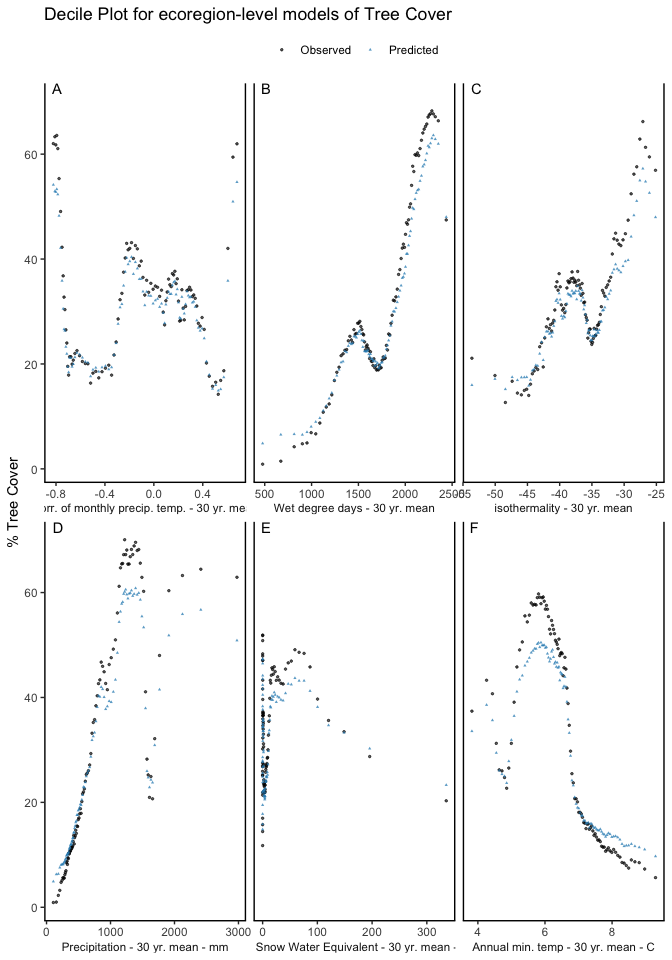
\includegraphics[keepaspectratio]{02_ModelFitting_files/figure-latex/decile_plot-1.pdf}}

\subsubsection{Deciles Filtered}\label{deciles-filtered}

20th and 80th percentiles for each climate variable

\begin{Shaded}
\begin{Highlighting}[]
\NormalTok{df }\OtherTok{\textless{}{-}}\NormalTok{ pred\_glm1[, prednames\_fig] }\CommentTok{\#\%\textgreater{}\% }
  \CommentTok{\#mutate(MAT = MAT {-} 273.15) \# k to c}
\FunctionTok{map}\NormalTok{(df, quantile, }\AttributeTok{probs =} \FunctionTok{c}\NormalTok{(}\FloatTok{0.2}\NormalTok{, }\FloatTok{0.8}\NormalTok{), }\AttributeTok{na.rm =} \ConstantTok{TRUE}\NormalTok{)}
\end{Highlighting}
\end{Shaded}

\begin{verbatim}
## $isothermality
##       20%       80% 
## -41.50744 -34.29430 
## 
## $sand
##      20%      80% 
## 38.64816 58.69292 
## 
## $AWHC
##       20%       80% 
##  8.315324 15.748090 
## 
## $t_warm_anom
##        20%        80% 
## -1.0562663  0.1251232 
## 
## $t_cold_anom
##        20%        80% 
## -1.3985424  0.2746704 
## 
## $prcp
##      20%      80% 
## 270.7078 432.6731 
## 
## $frostFreeDays_5_anom
## 20% 80% 
## -31  -3 
## 
## $isothermality_anom
##        20%        80% 
## -1.6492249  0.3364161 
## 
## $prcp_seasonality
##       20%       80% 
## 0.7864626 1.0409938 
## 
## $VPD_max
##      20%      80% 
## 1.116531 1.225946 
## 
## $prcpTempCorr_anom
##        20%        80% 
## -0.0909779  0.1553961 
## 
## $coarse
##       20%       80% 
##  3.139538 17.394847
\end{verbatim}

Filtered `Decile' plots of data. These plots show each vegetation
variable, but only based on data that falls into the upper and lower two
deciles of each predictor variable.

\begin{Shaded}
\begin{Highlighting}[]
\NormalTok{pred\_glm1\_deciles\_filt }\OtherTok{\textless{}{-}} \FunctionTok{predvars2deciles}\NormalTok{( pred\_glm1, }
                         \AttributeTok{response\_vars =}\NormalTok{ response\_vars,}
                         \AttributeTok{pred\_vars =}\NormalTok{ prednames\_fig,}
                         \AttributeTok{filter\_var =} \ConstantTok{TRUE}\NormalTok{,}
                         \AttributeTok{filter\_vars =}\NormalTok{ prednames\_fig) }

\FunctionTok{decile\_dotplot\_filtered\_pq}\NormalTok{(pred\_glm1\_deciles\_filt, }\AttributeTok{xvars =}\NormalTok{ prednames\_fig)}
\end{Highlighting}
\end{Shaded}

\pandocbounded{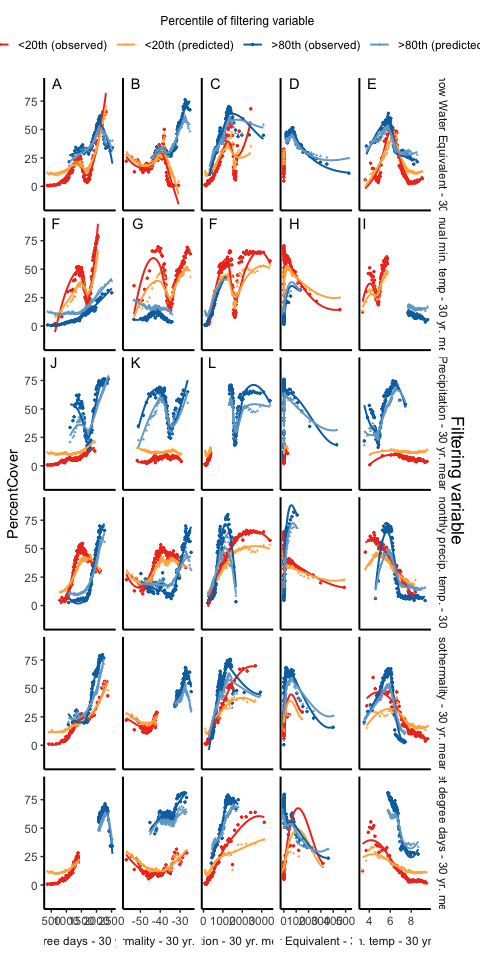
\includegraphics[keepaspectratio]{02_ModelFitting_files/figure-latex/glm_deciles_filtered-1.pdf}}

\begin{Shaded}
\begin{Highlighting}[]
\CommentTok{\#decile\_dotplot\_filtered\_pq(pred\_glm1\_deciles\_filt)}
\end{Highlighting}
\end{Shaded}

Filtered quantile figure with middle 2 deciles also shown

\begin{Shaded}
\begin{Highlighting}[]
\NormalTok{pred\_glm1\_deciles\_filt\_mid }\OtherTok{\textless{}{-}} \FunctionTok{predvars2deciles}\NormalTok{(pred\_glm1, }
                         \AttributeTok{response\_vars =}\NormalTok{ response\_vars,}
                         \AttributeTok{pred\_vars =}\NormalTok{ prednames\_fig,}
                         \AttributeTok{filter\_vars =}\NormalTok{ prednames\_fig,}
                         \AttributeTok{filter\_var =} \ConstantTok{TRUE}\NormalTok{,}
                         \AttributeTok{add\_mid =} \ConstantTok{TRUE}\NormalTok{)}

\NormalTok{g }\OtherTok{\textless{}{-}} \FunctionTok{decile\_dotplot\_filtered\_pq}\NormalTok{(}\AttributeTok{df =}\NormalTok{ pred\_glm1\_deciles\_filt\_mid, }\AttributeTok{xvars =}\NormalTok{ prednames\_fig)}
\NormalTok{g}
\end{Highlighting}
\end{Shaded}

\pandocbounded{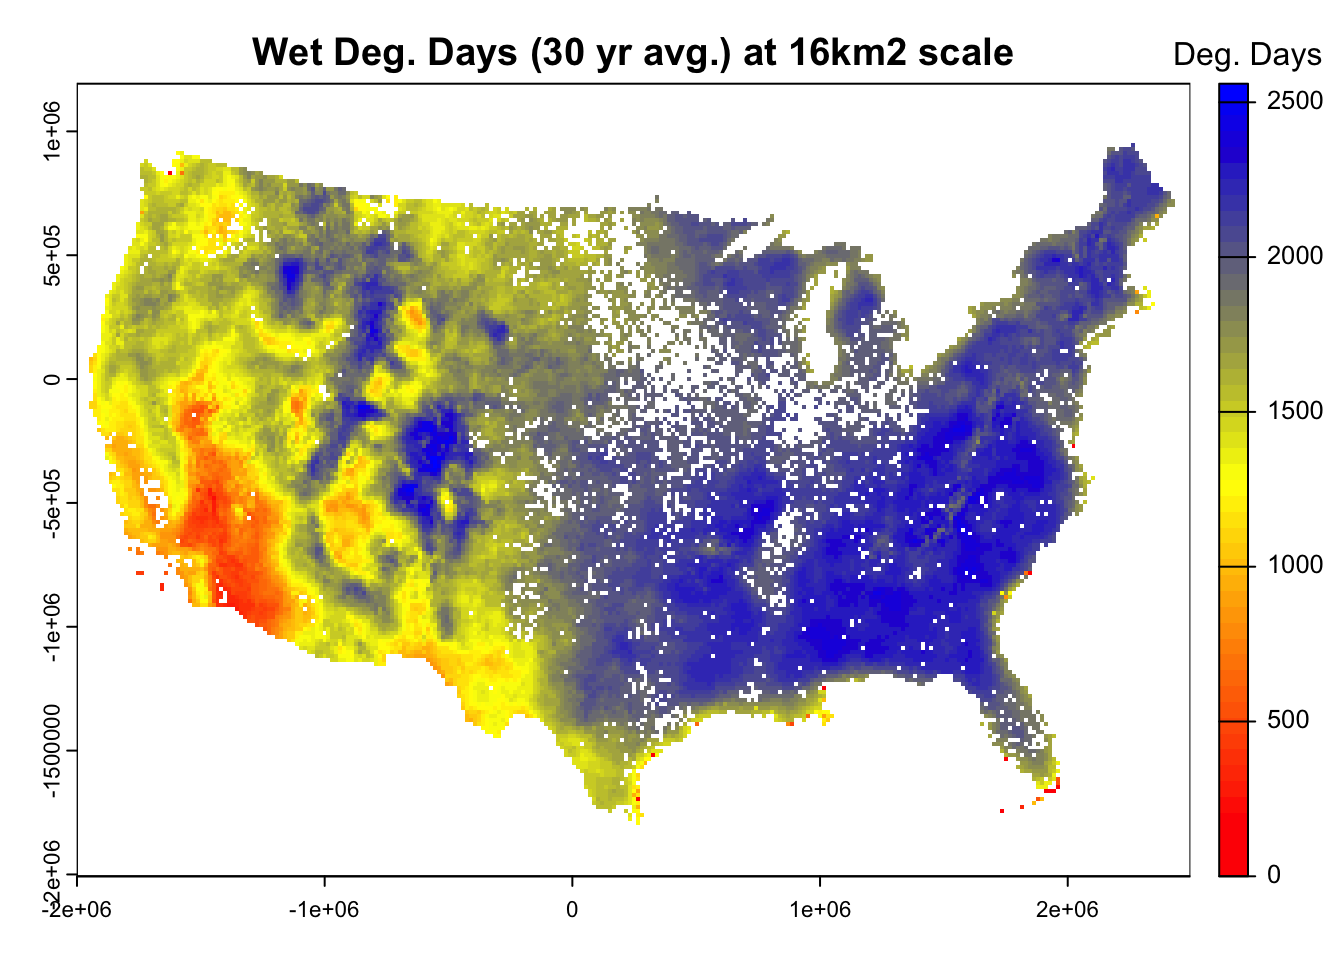
\includegraphics[keepaspectratio]{02_ModelFitting_files/figure-latex/unnamed-chunk-6-1.pdf}}

\begin{Shaded}
\begin{Highlighting}[]
\ControlFlowTok{if}\NormalTok{(save\_figs) \{x}
\FunctionTok{jpeg}\NormalTok{(}\FunctionTok{paste0}\NormalTok{(}\StringTok{"figures/quantile\_plots/quantile\_plot\_filtered\_mid\_v1"}\NormalTok{, s, }\StringTok{".jpeg"}\NormalTok{),}
     \AttributeTok{units =} \StringTok{"in"}\NormalTok{, }\AttributeTok{res =} \DecValTok{600}\NormalTok{, }\AttributeTok{width =} \FloatTok{5.5}\NormalTok{, }\AttributeTok{height =} \DecValTok{6}\NormalTok{ )}
\NormalTok{  g }
\FunctionTok{dev.off}\NormalTok{()}
\NormalTok{\}}
\end{Highlighting}
\end{Shaded}

\section{Save output}\label{save-output}

\begin{Shaded}
\begin{Highlighting}[]
\CommentTok{\# \# glm models}
\CommentTok{\# \#mods2save \textless{}{-} butcher::butcher(mod\_glmFinal) \# removes some model components so the saved object isn\textquotesingle{}t huge}
\CommentTok{\# }
\CommentTok{\# \#mods2save$formula \textless{}{-} best\_form}
\CommentTok{\# \#mods2save$pred\_vars\_inter \textless{}{-} pred\_vars\_inter \# so have interactions}
\CommentTok{\# \#n \textless{}{-} nrow(df\_sample)}
\CommentTok{\# \#mods2save$data\_rows \textless{}{-} n}
\CommentTok{\# }
\CommentTok{\# }
\CommentTok{\# if(!test\_run) \{}
\CommentTok{\#   saveRDS(mods2save, }
\CommentTok{\#         paste0("./models/glm\_beta\_model\_CONUSwide\_", s, "\_n", n, }
\CommentTok{\#         \#sample\_group, }
\CommentTok{\#         ".RDS"))}
\CommentTok{\#   if (byRegion == TRUE) \{}
\CommentTok{\#     \#\# western forests}
\CommentTok{\#      saveRDS(mods2save\_WF, }
\CommentTok{\#         paste0("./models/glm\_beta\_model\_WesternForests\_", s, "\_n", n, }
\CommentTok{\#         \#sample\_group, }
\CommentTok{\#         ".RDS"))}
\CommentTok{\#     \#\# eastern forests}
\CommentTok{\#      saveRDS(mods2save\_EF, }
\CommentTok{\#         paste0("./models/glm\_beta\_model\_EasternForests\_", s, "\_n", n, }
\CommentTok{\#         \#sample\_group, }
\CommentTok{\#         ".RDS"))}
\CommentTok{\#      \#\# grass/shrub}
\CommentTok{\#      saveRDS(mods2save\_G, }
\CommentTok{\#         paste0("./models/glm\_beta\_model\_GrassShrub\_", s, "\_n", n, }
\CommentTok{\#         \#sample\_group, }
\CommentTok{\#         ".RDS"))}
\CommentTok{\#   \}}
\CommentTok{\# \}}
\end{Highlighting}
\end{Shaded}

\begin{Shaded}
\begin{Highlighting}[]
\DocumentationTok{\#\# partial dependence plots}
\CommentTok{\#vip::vip(mod\_glmFinal, num\_features = 15)}

\CommentTok{\#pdp\_all\_vars(mod\_glmFinal, mod\_vars = pred\_vars, ylab = \textquotesingle{}probability\textquotesingle{},train = df\_small)}

\CommentTok{\#caret::varImp(fit)}
\end{Highlighting}
\end{Shaded}

\section{session info}\label{session-info}

Hash of current commit (i.e.~to ID the version of the code used)

\begin{Shaded}
\begin{Highlighting}[]
\FunctionTok{system}\NormalTok{(}\StringTok{"git rev{-}parse HEAD"}\NormalTok{, }\AttributeTok{intern=}\ConstantTok{TRUE}\NormalTok{)}
\end{Highlighting}
\end{Shaded}

\begin{verbatim}
## [1] "f861a83332ed5f906d36dc437452d8df7ce6f6e0"
\end{verbatim}

Packages etc.

\begin{Shaded}
\begin{Highlighting}[]
\FunctionTok{sessionInfo}\NormalTok{()}
\end{Highlighting}
\end{Shaded}

\begin{verbatim}
## R version 4.4.0 (2024-04-24)
## Platform: aarch64-apple-darwin20
## Running under: macOS Sonoma 14.6.1
## 
## Matrix products: default
## BLAS:   /Library/Frameworks/R.framework/Versions/4.4-arm64/Resources/lib/libRblas.0.dylib 
## LAPACK: /Library/Frameworks/R.framework/Versions/4.4-arm64/Resources/lib/libRlapack.dylib;  LAPACK version 3.12.0
## 
## locale:
## [1] en_US.UTF-8/en_US.UTF-8/en_US.UTF-8/C/en_US.UTF-8/en_US.UTF-8
## 
## time zone: America/Denver
## tzcode source: internal
## 
## attached base packages:
## [1] stats     graphics  grDevices utils     datasets  methods   base     
## 
## other attached packages:
##  [1] ggpubr_0.6.0       RColorBrewer_1.1-3 glmnet_4.1-8       Matrix_1.7-0      
##  [5] kableExtra_1.4.0   rsample_1.2.1      here_1.0.1         StepBeta_2.1.0    
##  [9] ggtext_0.1.2       knitr_1.49         gridExtra_2.3      pdp_0.8.2         
## [13] GGally_2.2.1       lubridate_1.9.4    forcats_1.0.0      stringr_1.5.1     
## [17] dplyr_1.1.4        purrr_1.0.4        readr_2.1.5        tidyr_1.3.1       
## [21] tibble_3.2.1       tidyverse_2.0.0    caret_6.0-94       lattice_0.22-6    
## [25] ggplot2_3.5.1      sf_1.0-16          tidyterra_0.6.1    terra_1.8-21      
## [29] glinternet_1.0.12  dtplyr_1.3.1       patchwork_1.3.0   
## 
## loaded via a namespace (and not attached):
##   [1] rstudioapi_0.17.1    shape_1.4.6.1        magrittr_2.0.3      
##   [4] modeltools_0.2-23    farver_2.1.2         rmarkdown_2.29      
##   [7] vctrs_0.6.5          rstatix_0.7.2        htmltools_0.5.8.1   
##  [10] curl_6.2.1           broom_1.0.7          Formula_1.2-5       
##  [13] pROC_1.18.5          parallelly_1.37.1    KernSmooth_2.23-22  
##  [16] plyr_1.8.9           sandwich_3.1-0       zoo_1.8-12          
##  [19] uuid_1.2-1           commonmark_1.9.1     lifecycle_1.0.4     
##  [22] iterators_1.0.14     pkgconfig_2.0.3      R6_2.6.1            
##  [25] fastmap_1.2.0        future_1.33.2        digest_0.6.37       
##  [28] colorspace_2.1-1     furrr_0.3.1          rprojroot_2.0.4     
##  [31] labeling_0.4.3       timechange_0.3.0     mgcv_1.9-1          
##  [34] abind_1.4-8          httr_1.4.7           compiler_4.4.0      
##  [37] proxy_0.4-27         aod_1.3.3            withr_3.0.2         
##  [40] backports_1.5.0      carData_3.0-5        betareg_3.1-4       
##  [43] DBI_1.2.3            ggstats_0.9.0        ggsignif_0.6.4      
##  [46] MASS_7.3-60.2        lava_1.8.0           rappdirs_0.3.3      
##  [49] classInt_0.4-10      gtools_3.9.5         ModelMetrics_1.2.2.2
##  [52] tools_4.4.0          units_0.8-5          lmtest_0.9-40       
##  [55] future.apply_1.11.2  nnet_7.3-19          glue_1.8.0          
##  [58] nlme_3.1-164         gridtext_0.1.5       grid_4.4.0          
##  [61] reshape2_1.4.4       generics_0.1.3       recipes_1.1.0       
##  [64] gtable_0.3.6         tzdb_0.4.0           class_7.3-22        
##  [67] data.table_1.17.0    hms_1.1.3            xml2_1.3.7          
##  [70] car_3.1-2            flexmix_2.3-19       markdown_1.13       
##  [73] foreach_1.5.2        pillar_1.10.1        splines_4.4.0       
##  [76] survival_3.5-8       tidyselect_1.2.1     svglite_2.1.3       
##  [79] stats4_4.4.0         xfun_0.51            hardhat_1.4.0       
##  [82] timeDate_4032.109    stringi_1.8.4        yaml_2.3.10         
##  [85] evaluate_1.0.3       codetools_0.2-20     cli_3.6.4           
##  [88] rpart_4.1.23         systemfonts_1.2.1    munsell_0.5.1       
##  [91] Rcpp_1.0.14          globals_0.16.3       parallel_4.4.0      
##  [94] gower_1.0.1          listenv_0.9.1        viridisLite_0.4.2   
##  [97] tigris_2.1           ipred_0.9-15         scales_1.3.0        
## [100] prodlim_2024.06.25   e1071_1.7-14         combinat_0.0-8      
## [103] rlang_1.1.5          cowplot_1.1.3
\end{verbatim}

\end{document}
